\documentclass[a4paper,fleqn]{cas-sc}

\usepackage[numbers]{natbib}
\usepackage{listings}
\usepackage{url}
\usepackage{booktabs}
\usepackage{graphicx}
\usepackage{caption}
\usepackage{float}
\usepackage[section]{placeins}
\usepackage{subcaption}
\usepackage{xcolor}
\captionsetup[table]{width=\textwidth}

\lstdefinestyle{Matlab-editor}{
  language=Matlab,
  basicstyle=\ttfamily\small,
  keywordstyle=\color{blue}\bfseries,
  commentstyle=\color{green!50!black},
  stringstyle=\color{red},
  numbers=left,
  numberstyle=\tiny,
  breaklines=true,
  frame=single
}

\begin{document}

\shorttitle{UrbanMobility-Instruct}
\shortauthors{Lin}

\title[mode=title]{UrbanMobility-Instruct: A Dataset-Centric Instruction Benchmark for Grounded Reasoning over Transportation Data}

\author[1]{Yufei Lin}
\cormark[1]
\ead{yufeilin@bennington.edu}

\affiliation[1]{organization={Bennington College},
            city={Bennington},
            state={Vermont},
            country={USA}}

\cortext[cor1]{Corresponding author.}

\begin{abstract}
Large language models (LLMs) have demonstrated strong reasoning and instruction-following capabilities, yet their application to urban science remains limited by the lack of domain-specific instruction datasets grounded in real-world urban data. This paper introduces a dataset-centric instruction-tuning framework that transforms heterogeneous urban mobility and infrastructure datasets into structured question-answering tasks for urban reasoning. The proposed corpus integrates five representative urban datasets and organizes instructions into three difficulty levels ranging from direct dataset comprehension to cross-dimensional reasoning. To improve robustness and diversity, the dataset incorporates contrastive positive--negative supervision and large-scale GPT-5.1-based augmentation, yielding 14,726 validated answer-generation records and 29,452 positive--negative answer-verification records across the five primary and two cross-regional sources. We evaluate the effectiveness of the dataset through supervised fine-tuning of representative models from the BERT, T5, LLaMA3, and Qwen families and further assess cross-regional generalization using transportation datasets from France and Japan. Experimental results reveal substantial architectural differences in adaptation behavior. Qwen models maintain near-perfect classification accuracy before and after fine-tuning, LLaMA3 models achieve the largest gains in dataset-grounded reasoning accuracy, and T5-base exhibits strong improvements in semantic generation despite persistent difficulties with structured answer selection. Cross-regional experiments demonstrate that dataset-centric reasoning transfers effectively across geographic contexts, although output-format compliance remains a significant challenge. These findings highlight the importance of dataset design in developing reliable, interpretable, and transferable LLMs for urban planning and transportation applications.
\end{abstract}

\begin{keywords}
large language models \sep instruction tuning \sep urban computing \sep transportation data \sep urban mobility \sep cross-regional generalization
\end{keywords}

\maketitle

\section{Introduction}\label{sec1}

Urban planning plays a critical role in shaping efficient, sustainable, and resilient cities. As rapid urbanization intensifies pressure on mobility systems, infrastructure, and environmental quality, planners increasingly rely on data-driven tools to support decision-making \cite{zheng2020urban, yeh2020urban}. Modern sensing technologies, ranging from ubiquitous traffic cameras to comprehensive Internet of Things (IoT) infrastructures, continuously generate large volumes of multimodal urban data describing human mobility, transportation behavior, emission levels, land-use patterns, and other indicators relevant to urban planning and management \cite{zhang2023urban, xu2022survey}. Despite their richness, these data sources are highly heterogeneous and fragmented, often differing substantially in structure, spatial and temporal resolution, metadata conventions, and analytical purpose. Extracting useful knowledge from them therefore requires considerable domain expertise and dataset-specific interpretation \cite{li2021survey, martinez2020data}. These challenges motivate the development of artificial intelligence (AI) systems capable of interpreting heterogeneous urban data and making the resulting information more accessible to planners, researchers, and policymakers.

Large language models (LLMs) have recently emerged as promising tools for analysis, reasoning, and interactive decision support. Their ability to synthesize information, interpret natural-language instructions, and generate context-aware responses has encouraged their application across a growing range of urban and transportation problems. Existing studies have explored LLMs for participatory urban design through agent-based systems \cite{zhou2024llm}, automated planning support \cite{zhu2024plangpt}, and disaster-related analysis \cite{zhu2024survey}. More specialized applications are also beginning to connect language models with urban mobility and spatial information. Liang et al.~\cite{liang2024mobility}, for example, investigate LLMs for human-mobility prediction under public events, illustrating how contextual event information can contribute to mobility analysis. LLMs have also been used to derive geographically meaningful representations from large-scale social-media text \cite{berragan2024semantic} and, when combined with multisource spatial information, to reason about fine-grained characteristics of the built environment such as walkability \cite{ki2025walkability}. At a broader level, systematic evaluations across hundreds of urban-planning tasks have begun to characterize both the capabilities and limitations of contemporary LLMs in urban decision-making contexts \cite{zhao2025urbanplanning}. Collectively, these developments demonstrate the growing potential of language models to support urban prediction, spatial interpretation, and planning-oriented reasoning.

Parallel advances in retrieval-augmented generation (RAG) and multi-agent LLM systems have further expanded this potential. RAG architectures can supplement model knowledge by retrieving relevant information from external sources such as zoning regulations, accident reports, planning documents, and infrastructure records \cite{lewis2020rag}. Multi-agent frameworks, meanwhile, can represent interactions among residents, vehicles, buildings, planners, and other urban stakeholders, enabling researchers to simulate collective behavior, evaluate planning interventions, and explore participatory decision-making \cite{zhou2024llm, park2023generative}. These approaches improve access to external information and enable richer forms of interaction, but they do not by themselves provide models with systematic knowledge of how heterogeneous urban datasets are structured or how their variables should be interpreted. A model may retrieve a transportation record or participate in an urban simulation while still lacking an explicit understanding of dataset-specific attributes, spatial and temporal relationships, physical constraints, and the connections among different urban data sources.

This distinction exposes an important gap in current LLM-based urban research. Much of the existing literature focuses on applying or evaluating general-purpose models on particular downstream tasks, whereas comparatively less attention has been devoted to constructing domain-specific instruction resources that explicitly teach models how to interpret real-world urban datasets. This limitation is particularly important because urban analysis frequently requires reasoning across heterogeneous sources rather than processing natural-language documents alone. Transportation trajectories, road-network structures, trip records, mobility statistics, and infrastructure data encode information through different schemas, scales, and relationships. General-purpose LLMs are not explicitly trained to reconcile these representations and may therefore lack the spatial, temporal, and domain grounding required for reliable urban analysis \cite{montoya2023urbanai, liu2023review}. Recent research has consequently emphasized the need for domain-adapted models capable of reasoning about mobility networks, road hierarchies, zoning structures, and broader urban-system dynamics \cite{xu2024llmurban, park2024llm4city}.

Instruction tuning provides a natural mechanism for addressing this gap. By transforming domain knowledge into structured instruction--response examples, models can be explicitly trained to recognize relevant concepts, interpret relationships among variables, and perform progressively more complex reasoning. Structured instruction formats have been shown to improve task adaptation and generalization across diverse domains \cite{wang2022supernaturalinstructions, longpre2023flan}, while domain-specific fine-tuning can improve factual reliability and reduce errors when models encounter specialized knowledge \cite{chung2022scaling, zhou2023lima}. For urban science, however, realizing these benefits requires more than converting planning documents into natural-language prompts. Instruction instances must remain grounded in authoritative urban datasets and preserve the semantics, statistical properties, and relationships represented by the underlying data.

To address this need, we introduce a dataset-centric instruction-tuning framework that transforms heterogeneous urban mobility and infrastructure data into structured question-answering tasks for urban reasoning. The proposed corpus integrates five representative sources: highD \cite{highd2024dataset}, NGSIM \cite{ngsim2024dataset}, the Road Networks dataset \cite{networkrepository2024road}, NYC Taxi and Limousine Commission (TLC) Trip Records \cite{nyc2024tlc}, and an urban flow prediction study \cite{wang2019optimal}. Rather than treating these sources as isolated collections, the framework organizes their information into a common instruction schema and three levels of reasoning difficulty, ranging from direct dataset comprehension to multi-attribute and cross-dimensional reasoning. The resulting tasks include both multiple-choice and short-answer formats and incorporate contrastive positive--negative supervision and large-scale augmentation to increase task diversity while preserving grounding in the source data. In this way, the framework shifts the role of urban datasets from passive information sources to explicit supervision for teaching models how to reason about urban systems.

We evaluate the resulting instruction corpus through supervised fine-tuning of representative models from the BERT, T5, LLaMA~3, and Qwen families, allowing us to examine how different model architectures and scales respond to dataset-grounded urban instruction tuning. The evaluation compares baseline and post-tuning performance across structured answer selection and semantic generation tasks. To further examine whether the learned reasoning patterns transfer beyond the regions represented in the primary corpus, we conduct cross-regional experiments using transportation datasets from France and Japan. This evaluation provides a test of whether instruction tuning based primarily on U.S.-centric urban data can support reasoning in environments characterized by different transportation systems, infrastructure, and mobility patterns.

\paragraph{Our Contributions.}
The main contributions of this work are summarized as follows:

\begin{itemize}

    \item \textbf{A question-answering focus, multi-level instruction-tuning dataset for urban science}. 
   We introduce a question-answering formatted dataset with three difficulty levels: Level~1 direct factual queries, Level~2 multi-attribute reasoning, and Level~3 cross-dataset and inferential reasoning. The dataset includes both multiple-choice and short-answer tasks, enabling progressively finer-grained reasoning capabilities. Built on this QA structure, we construct a unified instruction-tuning dataset that integrates five representative urban datasets and surveys, including highD, NGSIM, Road Networks, TLC Trip data, and urban flow prediction studies. By transforming heterogeneous urban mobility and infrastructure data into a coherent, instruction-driven benchmark, this contribution addresses long-standing fragmentation and accessibility challenges in urban science research \cite{zheng2014urban, batty2013new}, while aligning with evidence that structured instruction tuning improves reasoning quality and generalization in large language models \cite{longpre2023flan, wang2022supernaturalinstructions}.

   \item \textbf{Dataset construction pipeline setup for urban science instruction tuning}. We propose a four-stage pipeline that transforms heterogeneous urban datasets into a unified instruction-tuning resource. \textbf{Step~1} defines a multi-level difficulty hierarchy and complementary analytical perspectives, structuring urban science knowledge into progressively complex reasoning tasks. \textbf{Step~2} specifies a unified instruction schema with explicitly paired positive and negative examples to support supervised alignment. \textbf{Step~3} grounds each instruction in the original urban datasets, ensuring factual traceability and domain correctness. \textbf{Step~4} applies large-scale data augmentation to expand linguistic diversity and task coverage while preserving semantic and factual consistency. These four steps produce a instruction-tuning dataset that enables large language models to effectively learn urban science concepts and perform multi-attribute reasoning for downstream analytical and planning tasks.
    
    \item \textbf{Cross-model and cross-regional evaluation of urban science instruction tuning}. We evaluate the proposed instruction set across multiple model families—LLaMA~3, BERT, T5, and Qwen—spanning diverse architectural paradigms and model scales under a unified experimental protocol. The evaluation first assesses each model’s baseline performance on urban science tasks, followed by instruction tuning and post-tuning comparison to quantify performance gains and post-tuning comparison to quantify performance gains and reasoning transfer. To examine global adaptability, we conduct cross-regional generalization experiments using instruction datasets constructed via the proposed pipeline from transportation data in France and Japan, evaluating knowledge transfer across regions with distinct infrastructural and traffic characteristics. This process demonstrates the effectiveness of the instruction set in improving urban science reasoning across architectures and model sizes, while supporting robust cross-city and cross-regional generalization.

\end{itemize}

\section{Related Work}
\label{sec:related-work}

\subsection{Large Language Models}

Early transformer-based language models marked the beginning of modern NLP innovation. Encoder-only architectures such as BERT introduced deep bidirectional contextualization to support a wide range of language understanding tasks \cite{devlin2019bert}, while later encoder--decoder models---including BART and T5---extended this paradigm by unifying text-to-text pretraining and enabling both understanding and generation within a single framework \cite{lewis2020bart,raffel2020t5}. These model families established complementary strengths: BERT-style models excel at structured representation learning and classification, whereas T5-style architectures provide a flexible interface for unified generation and reasoning. As a result, both encoder-only and encoder--decoder models remain widely used backbones in domain-adaptive and instruction-based settings.

The next major shift was the rise of large decoder-only generative foundation models. GPT-3 demonstrated that scaling autoregressive transformers enables strong zero-shot and few-shot performance across diverse tasks \cite{brown2020gpt3}, motivating subsequent research on scaling laws that formalized the relationship between model capacity, data volume, and compute \cite{kaplan2020scaling}. Building on these insights, the LLaMA family introduced efficient, open-weight large language models designed for research and downstream fine-tuning \cite{touvron2023llama2}. LLaMA~2 further expanded this line with larger-scale pretraining, improved safety alignment, and instruction-tuned variants suitable for supervised fine-tuning and preference optimization \cite{touvron2023llama2}. More recently, LLaMA~3 advanced model scale, multilingual coverage, and reasoning performance, reinforcing the role of open-source LLMs as competitive foundations for applied and scientific domains \cite{meta2024llama3}.

In parallel, the Qwen family represents another influential line of open large language models optimized for multilingual and instruction-following performance. Qwen models adopt a decoder-only transformer architecture similar to GPT and LLaMA, but emphasize large-scale multilingual corpora, strong code and reasoning capabilities, and explicit instruction tuning across diverse task formats \cite{bai2023qwen}. Subsequent releases, including Qwen2 and Qwen2.5, further improved long-context modeling, reasoning robustness, and alignment, making Qwen a strong alternative backbone for cross-domain and cross-lingual instruction learning \cite{qwen2024technical}. The inclusion of Qwen models alongside LLaMA enables a more comprehensive evaluation across open-source generative LLM ecosystems.

Together, these three architectural families---encoder-only (BERT), encoder--decoder (T5), and decoder-only generative models (LLaMA and Qwen)---form the backbone selection used in our experimental evaluation. Their complementary design philosophies allow us to systematically examine how architectural choices interact with instruction design, supervision signals, and domain-specific data.

While these pretrained models exhibit strong general-purpose language capabilities, their performance in specialized domains such as urban planning and transportation analysis remains limited without targeted adaptation. Recent work has shown that instruction fine-tuning with carefully constructed, domain-grounded datasets can substantially improve reasoning accuracy and reduce hallucinations in technical tasks \cite{wei2022finetuned,chung2022scaling}. Motivated by these findings, our work focuses on systematically fine-tuning representative models from each architectural family on a curated urban-science instruction dataset, enabling controlled evaluation across model types, regions, and task levels.


\subsection{Instruction Tuning}

Instruction tuning was introduced to improve the generalization and usability of large language models by explicitly training them to follow natural language instructions. Early frameworks such as T0 and Super-NaturalInstructions demonstrated that multi-task prompted training enables zero-shot generalization to unseen tasks by treating task descriptions as first-class supervision signals \cite{sanh2022t0,mishra2022supernatural}. The FLAN collection further scaled this paradigm, showing that large, diverse, and carefully curated instruction sets substantially enhance zero-shot and few-shot performance across a wide range of benchmarks \cite{longpre2023flan}. In parallel, InstructGPT and subsequent alignment-focused work formalized instruction following with human feedback, emphasizing the importance of aligning model outputs with user intent and expectations for downstream usability \cite{ouyang2022training}. More recent analyses, including prompt-loss–based fine-tuning, have refined our understanding of how different instruction-tuning objectives influence robustness and generalization \cite{huerta2024instruction}. Despite these advances, broad instruction datasets often struggle with highly domain-specific tasks—such as those requiring geospatial reasoning, specialized data schemas, or regulatory knowledge—highlighting limitations of general-purpose instruction tuning.

Beyond single-step instruction following, recent work has expanded instruction tuning toward multi-step reasoning and structured decision-making. Chain-of-thought prompting reveals latent reasoning capabilities by encouraging step-by-step explanations \cite{wei2022cot}, while frameworks such as ReAct integrate reasoning and action to support planning, tool use, and iterative problem solving \cite{yao2023react}. In parallel, synthetic instruction generation has emerged as a scalable alternative to manual annotation. Self-Instruct \cite{wang2023selfinstruct} demonstrates that LLMs can autonomously generate diverse, high-quality instruction prompts that significantly improve instruction-following performance. Alpaca-style approaches further show that a strong teacher model can be used to generate large volumes of synthetic instruction–response pairs that effectively train smaller models, while LIMA highlights that carefully curated synthetic data—even at relatively small scale—can achieve strong alignment and reasoning quality \cite{taori2023alpaca,zhou2023lima}. Collectively, these findings establish LLM-generated synthetic supervision as a practical and effective strategy for instruction tuning.

While instruction tuning has proven effective across general NLP tasks and model families—including T5, BERT variants, and LLaMA-based models \cite{wei2022finetuned}—most existing instruction datasets remain weakly grounded in domain-specific constraints. In particular, they rarely encode structured metadata, spatial–temporal heterogeneity, or cross-dimensional relationships characteristic of urban and transportation data. This gap motivates our focus on constructing a domain-aligned instruction dataset for urban planning, where instruction design, difficulty progression, and synthetic augmentation are explicitly grounded in real-world datasets and planning-relevant reasoning patterns.

The use of large language models for generating synthetic instruction data is well supported in prior research. Self-Instruct \cite{wang2023selfinstruct} demonstrates that LLMs can autonomously produce high-quality instructional prompts that significantly improve downstream instruction-following capabilities. Alpaca \cite{taori2023alpaca} further shows that a stronger model can be leveraged to generate large volumes of synthetic instruction–response pairs that effectively train smaller models. LIMA \cite{zhou2023lima} highlights that carefully curated synthetic data, even in relatively small quantities, can achieve high-quality alignment. These findings validate our use of GPT\mbox{-}5.1 to generate augmented variants for both short-answer and multiple-choice formats.

\subsection{LLMs and Instruction Dataset for Urban Computing}

Urban computing research has long integrated heterogeneous data sources to characterize city dynamics, with advances in GeoAI and spatial foundation models further extending the ability of computational systems to represent and reason about geographic information \cite{zheng2014urban,zheng2016urban,batty2013new,wang2024spatial,huang2022geoai}. Deep spatio-temporal models for traffic forecasting, including ST-GDN, ST-Norm, and cross-city transfer and meta-learning approaches, have demonstrated strong predictive capabilities while also revealing persistent difficulties in transferring spatial and temporal patterns across regions \cite{wang2020traffic,deng2021st,pan2019urban,zhang2020metast,lee2020crosscitytransfer}. More recently, geospatial language models such as GeoGPT have introduced natural-language interaction with spatial information \cite{gao2024geogpt}, extending urban computing from specialized predictive models toward more general systems capable of interpreting and reasoning about urban knowledge.

This transition has enabled language models to address an increasingly diverse range of urban tasks. Early computational approaches to large-scale urban text demonstrated the scalability of NLP and deep learning while highlighting the continuing importance of contextual knowledge when interpreting less structured urban information \cite{lore2024hybrid}. LLM-based methods have subsequently expanded this capability by connecting unstructured language with explicit geographic and spatial contexts. For example, language models have been used to derive geographically meaningful semantic representations from large-scale social-media text \cite{berragan2024semantic}, while GeoGPT and related systems enable natural-language reasoning over geospatial information \cite{gao2024geogpt}. Beyond textual and geographic interpretation, LLMs have also been applied to human-mobility prediction under public events, where contextual information can contribute to understanding changes in transportation behavior \cite{liang2024mobility}. Multimodal approaches further combine language-model reasoning with street-view imagery and multisource spatial data to characterize built-environment properties such as walkability \cite{ki2025walkability}. At the planning level, systems such as PlanGPT, UniST, and participatory planning agents extend language-model-based methods toward regulatory interpretation, urban forecasting, scenario analysis, and civic engagement \cite{zhu2024plangpt,yuan2024unist,zhou2024participatory,lin2024urbangovernance}. Systematic evaluation across hundreds of urban-planning tasks further demonstrates that contemporary LLMs possess substantial capabilities across this broad task space, while retaining notable weaknesses in spatial reasoning and specialized professional knowledge \cite{zhao2025urbanplanning}.

Taken together, these developments illustrate a progression from task-specific urban prediction and text analysis toward increasingly general language-based systems capable of interacting with geographic, mobility, multimodal, and planning information. However, the expansion of downstream capabilities does not necessarily provide models with a systematic understanding of the datasets underlying urban analysis. Most existing approaches either apply general-purpose models directly to urban tasks or provide external information through documents, prompts, retrieval mechanisms, or multimodal inputs. Consequently, a model may perform a planning task or interpret a spatial observation without having been explicitly trained to understand how an urban dataset is organized, what its variables represent, how attributes relate to one another, or how reasoning patterns learned from one dataset may transfer to another geographic context. This distinction becomes particularly important when urban analysis involves heterogeneous traffic trajectories, road networks, trip records, infrastructure information, and other sources that differ substantially in schema, spatial scale, temporal resolution, and semantics.

Domain adaptation and fine-tuning offer a potential mechanism for addressing this limitation, and several recent efforts have constructed specialized training resources for urban applications. Zhang et al.~\cite{urbanclaim2025}, for example, construct a large-scale corpus from news articles across 113 Chinese cities and apply supervised classification to identify policy-related information. This approach demonstrates the value of domain-specific urban training data, but its supervision is designed primarily for policy classification rather than for teaching models to interpret the structure and relationships contained within urban datasets. CityGPT~\cite{citygpt2024} broadens domain adaptation by compiling city-related documents, planning reports, and municipal knowledge into instruction-style data for city-oriented question answering. Similarly, PlanGPT~\cite{plangpt2024} transforms planning activities such as zoning analysis, urban-design critique, and scenario exploration into structured instruction--response pairs, providing models with explicit supervision for planning-oriented reasoning.

These efforts represent an important shift from directly prompting general-purpose LLMs toward adapting models with urban-domain knowledge. Nevertheless, the information used for adaptation remains predominantly organized around documents, policies, domain questions, or downstream planning tasks. The underlying urban datasets themselves are rarely treated as the primary object of instruction. As a result, existing training resources provide limited explicit supervision for learning dataset schemas, metadata, variable semantics, statistical properties, and relationships among heterogeneous urban data sources. This leaves a gap between domain-aware language modeling and the dataset-level understanding required to perform reliable urban analysis.

Our work addresses this gap by treating urban dataset understanding as a fundamental instruction-tuning objective. Rather than constructing instructions primarily from policy documents or predefined planning tasks, we derive structured question--answer instances directly from the metadata, organization, descriptive properties, and relationships represented in heterogeneous urban mobility and infrastructure datasets. The resulting instruction corpus is organized into progressively more complex reasoning levels and combines multiple-choice and short-answer tasks to move from direct dataset comprehension toward multi-attribute and cross-dimensional reasoning. By further evaluating models across different architectures and transportation datasets from multiple geographic regions, we examine not only whether models can acquire dataset-grounded urban knowledge through instruction tuning, but also whether the resulting reasoning patterns transfer beyond the datasets and regions from which the primary instruction corpus is constructed.

\section{Method}\label{sec4}
\subsection{Motivation}
Our approach adapts the instruction-following framework introduced by Ouyang et al.~\cite{ouyang2022training}, which relies on high-quality supervised examples, paired positive and negative demonstrations, and systematic prompt diversification to enable pretrained models to respond to unseen instructions in a structured and methodical manner. While their framework is designed for broad, general-purpose tasks, our adaptation targets the domain of urban planning, aiming to teach models to reason as urban planners do by grounding their understanding in the properties, constraints, and analytical processes inherent to real-world urban datasets.

\subsection{Overview of Approach}


Guided by these observations, we construct a dataset-centric instruction corpus by examining five representative urban datasets: highD, NGSIM, Road Networks, NYC TLC Trip Records, and the Urban Flow Prediction Survey—and converting their core descriptive properties into short-answer and multiple-choice instructions. Each instruction is written in both positive and negative forms to provide contrastive supervision, and is assigned to one of three difficulty levels reflecting increasingly deeper forms of dataset understanding: Level~1 focuses on direct comprehension of basic dataset attributes, Level~2 targets reasoning over multiple related attributes within a dataset, and Level~3 requires cross-dimensional interpretation connecting different aspects of the data. After constructing the seed set, we use GPT\mbox{-}5.1 to generate large-scale augmented variants that remain factually grounded while introducing lexical and structural diversity. This final corpus is then used to fine-tune three major model families—LLaMA, BERT, and Qwen—to evaluate how dataset-grounded instruction tuning enables different architectures to acquire progressively more complex forms of urban reasoning.

\subsection{Dataset Construction}

The primary goal of our dataset is to equip language models with the ability to interpret the metadata, structure, and descriptive properties of real-world urban datasets, and to cultivate the foundational thinking skills that urban planners apply when working with empirical data. Whereas general-purpose instruction datasets focus on broad natural-language tasks, our intention is to train models to understand what an urban dataset contains, how it is collected, how its variables relate to one another, and how such information is used in practical planning contexts. By grounding the instructions directly in dataset metadata, measurement fields, and usage conventions, our dataset enables models to develop the systematic reasoning patterns necessary for interpreting urban data. This dataset-centric perspective provides the structural foundation required for downstream tasks such as urban analysis, forecasting, simulation, and decision support within planning workflows.

Our instruction corpus is constructed through a multi-stage pipeline that progressively transforms raw urban datasets into structured, contrastive training signals for large language models. The process consists of five core steps:
(1) defining difficulty levels to capture increasing reasoning depth,
(2) designing instruction schemas,
(3) extracting grounded information from source datasets,
(4) constructing positive–negative contrastive pairs, and
(5) performing large-scale data augmentation.
Each step is described in detail below.

\subsubsection{Step 1: Define Difficulty Levels}

To capture varying depths of dataset understanding, we categorize all instructions into three difficulty levels that reflect increasing reasoning complexity. This design is motivated by how urban planners interact with real-world datasets in practice, where reasoning typically progresses from basic factual validation, to integrated assessment of multiple dataset attributes, and finally to higher-level interpretation within broader urban-system contexts.

For example, consider a planner evaluating the NYC TLC Trip Records to study congestion dynamics in Manhattan. The planner must first verify fundamental properties of the dataset—such as temporal coverage, spatial granularity, and available trip-level variables—to ensure the data is suitable for analysis. Next, the planner must reason across multiple attributes, such as whether the combination of pickup–dropoff zone resolution and timestamp granularity supports peak-hour congestion analysis, or how fare variables interact with trip distance to infer travel conditions. Ultimately, the planner may interpret these observations in a broader urban context, connecting observed trip patterns to network structure, traveler behavior, or policy interventions such as congestion pricing. This progression—from factual comprehension, to multi-attribute synthesis, to cross-dimensional interpretation—forms the basis of our three-level instruction taxonomy.

\textbf{Level~1: Direct Dataset Comprehension.}
Level~1 focuses on factual understanding of a dataset’s core descriptive properties. To reflect the foundational knowledge required in everyday planning practice, we define ten key perspectives as the basis for Level~1 instruction design:
\begin{itemize}
\item Provenance,
\item Spatial coverage,
\item Temporal coverage,
\item Measurement resolution,
\item Variable definitions,
\item File structure,
\item Collection methodology,
\item Usage context,
\item Dataset limitations.
\end{itemize}
Tasks at this level require models to accurately identify or restate explicit metadata elements without additional reasoning. For each source dataset and each instruction format (short answer and multiple choice), we create one seed instruction per perspective, yielding 20 Level~1 seed instructions per dataset. These instructions establish the essential grounding required for higher-level reasoning.

\textbf{Level~2: Multi-Attribute Reasoning.}
Level~2 instructions require models to integrate two or more dataset attributes to derive a correct answer. Representative tasks include relating spatial extent to sampling frequency, connecting variable definitions with data-collection procedures, or interpreting how multiple metadata fields jointly characterize a dataset’s operational constraints. In the NYC TLC context, such reasoning may involve assessing whether zone-level pickup data combined with timestamp granularity is sufficient to distinguish localized congestion from citywide demand shifts. These tasks emulate intermediate analytical reasoning, where planners synthesize multiple components of a dataset to assess its applicability and limitations. For each source dataset, we select five meaningful combinations of Level~1 perspectives and, based on each combination, construct both short-answer and multiple-choice Level~2 seed instructions, resulting in five Level~2 seeds per dataset.

\textbf{Level~3: Cross-Dimensional Interpretation.}
Level~3 instructions involve reasoning that spans multiple facets of a dataset or connects dataset characteristics across broader conceptual dimensions. Examples include interpreting how traffic dynamics interact with temporal sampling schemes, aligning aggregated mobility indicators with structural properties of urban road networks, or relating observed trip patterns to behavioral responses and policy interventions. For the NYC TLC Trip Records, such tasks may require reasoning about how temporal variations in trip duration reflect underlying congestion dynamics, regulatory changes, or shifts in travel behavior rather than data artifacts alone. These tasks approximate higher-level planning cognition, where insights emerge from integrating multiple layers of urban information. For this level, we generate five short-answer seed instructions for datasets that naturally support such cross-dimensional reasoning, specifically the NYC TLC Trip Records and the Urban Flow Prediction Survey.

\subsubsection{Step 2: Instruction Schema}

To operationalize the difficulty levels, we design two complementary instruction schemas: \emph{short-answer} and \emph{multiple-choice}. Both schemas are applied consistently across all difficulty levels and are grounded in dataset metadata, documentation, and structural attributes.

Short-answer instructions require models to generate concise textual responses grounded in specific dataset properties, such as describing data-collection methods, stating spatial or temporal coverage, or explaining documented limitations. Multiple-choice instructions emphasize precise recognition and classification: each question provides four answer options (A–D) with a single correct choice, targeting clearly defined properties such as variable semantics, file organization, categorical attributes, or usage constraints.

Together, these schemas balance open-ended explanation with discrete decision-making, enabling models to learn both expressive reasoning and precise factual discrimination—two complementary capabilities essential for dataset-centric urban analysis.

\subsubsection{Step3: Source Datasets and Information Grounding}

We construct instructions using five representative datasets widely adopted in transportation engineering, mobility analysis, and urban planning research: highD, NGSIM, urban road network datasets, NYC TLC Trip Records, and the Urban Flow Prediction Survey. Each dataset contributes a distinct perspective on urban systems, ranging from microscopic vehicle trajectories to macroscopic mobility patterns and network-level infrastructure representations.

The highD and NGSIM datasets provide high-resolution vehicle trajectories from highway environments, supporting instructions related to sensing methodology, spatial–temporal resolution, and traffic behavior. Urban road network datasets offer graph-structured representations of road geometry and connectivity, enabling instructions on network topology, node–edge semantics, and infrastructure interpretation. The NYC TLC Trip Records dataset contributes rich metadata on taxi trips, fares, and temporal patterns, supporting reasoning about human mobility and demand dynamics. The Urban Flow Prediction Survey provides aggregated flow indicators, measurement protocols, and survey-based attributes relevant to forecasting and planning tasks.

All instructions are explicitly grounded in dataset documentation, metadata fields, or established dataset descriptions, ensuring factual accuracy and reproducibility.

\subsubsection{Step 4: Contrastive Positive–Negative Pairing}

To strengthen model robustness and reduce superficial pattern learning, we adopt a contrastive pairing strategy inspired by prior instruction-tuning work \cite{ouyang2022training}. Each instruction is instantiated in both a positive and a negative form.

In the positive variant, the output and explanation accurately reflect the underlying dataset. In the negative variant, the output is intentionally incorrect while the surrounding context and reasoning structure remain minimally altered. For multiple-choice tasks, the negative example replaces the correct answer with a plausible but incorrect alternative. For short-answer tasks, the negative example substitutes an incorrect textual response while preserving the original explanation format.

This contrastive setup teaches models not only how to produce correct interpretations of urban data, but also how to avoid realistic yet subtle misinterpretations that frequently arise in applied urban analysis.

\subsubsection{Step 5: Data Augmentation}

After constructing the seed instruction set, we employ GPT\mbox{-}5.1 to generate multiple grounded variants of the factual context, question, correct answer, explanation, and---for multiple-choice tasks---option ordering. The exact expansion factors depend on task type and difficulty level. After validation, the five primary sources contain 10,560 answer-generation records; the independently held-out France and Japan sources contribute another 4,166 records. Table~\ref{tab:dataset_by_level} reports the validated primary-source composition. Each canonical record additionally produces one positive and one negative answer-verification view.

\begin{table}[H]
\centering
\caption{Validated answer-generation records from the five primary sources, reported by difficulty level and task type. France and Japan are excluded because they are reserved as cross-regional holdouts.}
\label{tab:dataset_by_level}
\resizebox{\columnwidth}{!}{%
\renewcommand{\arraystretch}{1.15}
\begin{tabular}{lcccccc}
\toprule
\textbf{Data Source} &
\textbf{Level 1} &
\textbf{Level 2} &
\textbf{Level 3} &
\textbf{SA} &
\textbf{MC} &
\textbf{Total} \\
\midrule
highD &
1,520 &
510 &
0 &
715 &
1,315 &
2,030 \\

NGSIM &
1,520 &
510 &
0 &
715 &
1,315 &
2,030 \\

Road Networks &
1,520 &
510 &
0 &
715 &
1,315 &
2,030 \\

TLC Trip Records &
1,520 &
510 &
205 &
920 &
1,315 &
2,235 \\

Urban Flow Prediction Survey &
1,520 &
510 &
205 &
920 &
1,315 &
2,235 \\
\midrule

\textbf{Total} &
\textbf{7,600 (72.0\%)} &
\textbf{2,550 (24.1\%)} &
\textbf{410 (3.9\%)} &
\textbf{3,985 (37.7\%)} &
\textbf{6,575 (62.3\%)} &
\textbf{10,560} \\
\bottomrule
\end{tabular}
}
\end{table}

% \begin{table}[!h]
% \centering
% \large
% \caption{We intentionally allocate the majority of samples to Level 1 \& 2 for ground-\\-ing and compositional reasoning, while reserving a focused Level 3 subset to train\\ and evaluate cross-dimensional reasoning. The \textit{Total} column further reports the \\within-source task-type distribution between Short Answer (SA) and Multiple\\ Choice (MC).}
% \label{tab:dataset_by_level}
% \resizebox{\columnwidth}{!}{%
% \renewcommand{\arraystretch}{1.15} % small vertical gap between rows
% \begin{tabular}{p{2.8cm} p{2.3cm} p{2cm} p{2.2cm} p{3cm}}
% \toprule
% \textbf{Data Source} & \textbf{Level 1} & \textbf{Level 2} & \textbf{Level 3} & \textbf{Total} \\
% \midrule
% highD & 3{,}000 & 1{,}000 & 0     & \parbox[t]{4.6cm}{4{,}000\\SA 35.0\%\\MC 65.0\%\\} \\
% NGSIM & 3{,}000 & 1{,}000 & 0     & \parbox[t]{4.6cm}{4{,}000\\SA 35.0\%\\MC 65.0\%\\} \\
% Road Networks & 3{,}000 & 1{,}000 & 0 & \parbox[t]{4.6cm}{4{,}000\\SA 35.0\%\\MC 65.0\%\\} \\
% TLC Trip Records & 3{,}000 & 1{,}000 & 1{,}000 & \parbox[t]{4.6cm}{5{,}000\\SA 48.0\%\\MC 52.0\%\\} \\
% Urban Flow Prediction Survey & 3{,}000 & 1{,}000 & 1{,}000 & \parbox[t]{4.6cm}{5{,}000\\SA 48.0\%\\MC 52.0\%} \\
% \midrule
% \textbf{Total} & \textbf{15{,}000 (68.2\%)} & \textbf{5{,}000 (22.7\%)} & \textbf{2{,}000 (9.1\%)} & \parbox[t]{4.6cm}{\textbf{22{,}000\\SA 40.9\%\\MC 59.1\%}} \\
% \bottomrule
% \end{tabular}
% }
% \end{table}
% use light colors
\begin{figure}[H]
    \centering
    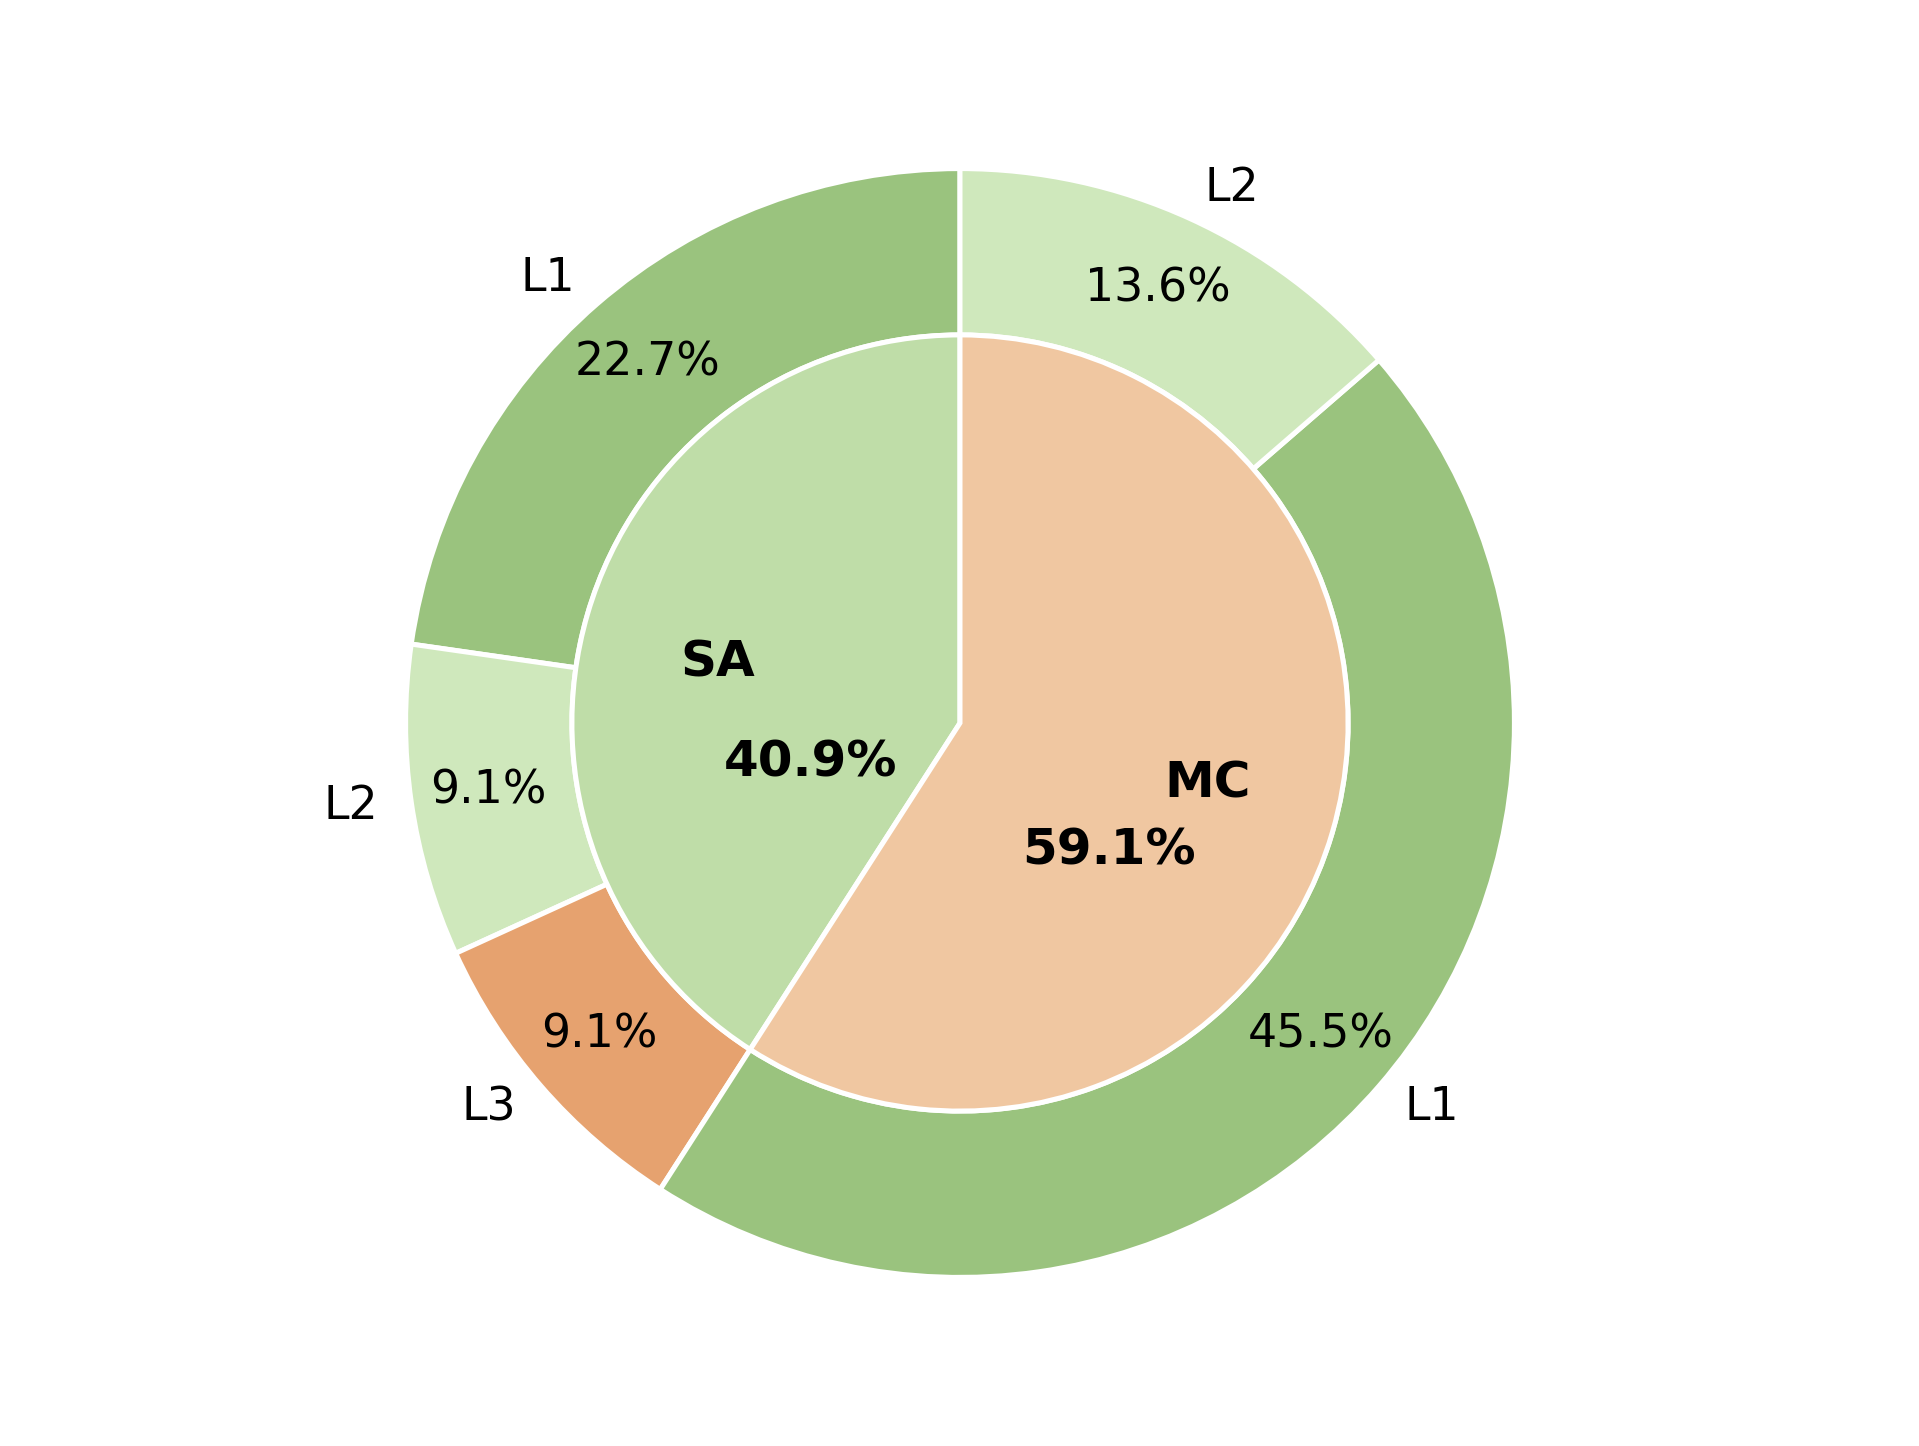
\includegraphics[width=\linewidth]{./graphs/sa_mc_levels_inner_fullpie_pro.png}
    \caption{Nested pie chart summarizing the augmented instruction dataset composition. The inner pie shows the overall task-type split between short-answer (SA) and multiple-choice (MC) instructions, while the outer ring breaks down reasoning difficulty within each task type: SA contains Level~1/Level~2/Level~3 instructions, whereas MC contains Level~1/Level~2 only (no Level~3 MC instances). \textit{Note:} across the full dataset, positive and negative instances are generated in a balanced 1:1 ratio (50\% positive, 50\% negative).}
\label{fig:sa_mc_level_distribution}
\end{figure}

% move to related work


During augmentation, GPT\mbox{-}5.1 rephrases factual descriptions, rewrites questions, varies explanation styles, and reorders multiple-choice options. For negative examples, it produces incorrect yet plausible outputs that remain compatible with the contextual constraints of each instruction. This strategy increases lexical and structural diversity, reduces template memorization, and strengthens the contrastive supervision signal.

Through systematic augmentation grounded in a small, curated set of seed instructions, the final dataset becomes a rich and varied training resource that enables models to generalize beyond fixed phrasings and develop robust dataset-grounded reasoning across all levels.

\subsubsection{Step 6: Lineage-Aware Validation and Leakage Auditing}

Synthetic expansion can create highly similar descendants of the same underlying question; consequently, a row-level random split would overestimate generalization by allowing paraphrases of a training example to enter validation or test data. We therefore retain explicit lineage for every record. Each manually authored item receives a deterministic \texttt{seed\_id}, and every original and augmented descendant inherits this identifier. In addition, items derived from the same normalized source fact---including multiple-choice, short-answer, positive-verification, and negative-verification forms---share a deterministic \texttt{concept\_group\_id}. Two pairs of semantically equivalent concepts identified during manual review were consolidated through a documented alias map before partitioning. Split assignment is performed on these resolved concept groups rather than on individual records, ensuring that all task-format and paraphrase variants of a concept remain in a single partition.

The pipeline next applies structural and task-specific quality controls. It validates required fields, answer--option consistency for multiple-choice records, answer grounding for short-answer records, and the separation of prompts from supervised targets. Exact duplicate records are removed, while plausible incorrect answers are used only to construct an answer-verification task; they are not treated as generation targets. This procedure yielded 14,726 accepted canonical records and an equal number of answer-generation views, together with 29,452 verification views containing balanced positive and negative candidates. No record was rejected by the final structural gate, and no exact duplicate remained.

We audit leakage at four levels: resolved concept-group overlap, seed overlap, normalized exact-prompt overlap, and semantic similarity across splits. The first three deterministic checks reported zero overlap for every train--validation--test pair. For the semantic audit, prompts were encoded with \texttt{all-mpnet-base-v2}, and cross-split pairs with cosine similarity of at least 0.90 were retained. Comparisons were deduplicated by concept pair before review so that many augmented variants did not produce repeated judgments. After the reviewed concept aliases were applied, three unique concept pairs remained. Manual adjudication classified all three as related but distinct because they required different answers or reasoning operations; none was confirmed as leakage. The final audit therefore contained zero pending and zero confirmed-leakage cases.

The process is demonstrated as the following Figure ~\ref{fig:urban_llm_flowchart}.

\begin{figure}[H]
    \centering
    
\includegraphics[width=\textwidth]{graphs/Data Construction Pipeline.png}
    \caption{End-to-end dataset construction pipeline for the proposed urban-planning instruction corpus. The workflow begins with five heterogeneous urban datasets and proceeds through seed instruction creation across three difficulty levels, contrastive positive/negative pairing, and large-scale GPT-5.1 augmentation. The final output is a comprehensive multi-level instruction dataset designed to train language models in structured, dataset-grounded urban reasoning.}
    \label{fig:urban_llm_flowchart}
\end{figure}

% \begin{figure}[!h]
%     \centering
%     
\includegraphics[width=\linewidth]{./graphs/Data Construction Pipeline.png}
%     \caption{End-to-end dataset construction pipeline for the proposed urban-planning instruction corpus. The workflow begins with five heterogeneous urban datasets and proceeds through seed instruction creation across three difficulty levels, contrastive positive/negative pairing, and large-scale GPT-5.1 augmentation. The final output is a comprehensive multi-level instruction dataset designed to train language models in structured, dataset-grounded urban reasoning.}
%     \label{fig:urban_llm_flowchart}
% \end{figure}

% \subsection{Models and Evaluation Design}

% \subsubsection{Model Selection}

% To assess the robustness of dataset-centric instruction tuning across architectures and model capacities, we select three representative language model families: \textbf{LLaMA}, \textbf{BERT}, and \textbf{Qwen}. These families cover decoder-only, encoder-based, and modern instruction-oriented architectures, respectively. For each model family, we evaluate \emph{three different model sizes}, enabling analysis of how model scale influences the acquisition of dataset-grounded urban reasoning skills in addition to architectural differences.

% \begin{table}[!ht]
% \centering
% \caption{Summary of model families selected for instruction tuning and evaluation.\\ LLaMA, BERT, and Qwen are chosen to represent three complementary architectural\\ paradigms—decoder-only generative models, encoder-only contextual representation\\ models, and modern large-scale decoder-only models, respectively. Evaluating across\\ these families allows us to examine how dataset-centric instruction tuning transfers\\ across fundamentally different model designs and learning biases. For each family, three\\ model sizes are tested to analyze the effect of model capacity on urban reasoning\\ performance, ensuring that observed improvements are not confined to a single architecture\\ or scale.\\}
% \label{tab:models_metrics}
% \resizebox{\columnwidth}{!}{%
% \begin{tabular}{|p{2.5cm}|p{3cm}|p{4cm}|}
% \hline
% \textbf{Model Family} & \textbf{Architecture Type} & \textbf{Primary Task Focus} \\ \hline
% LLaMA & Decoder-only Transformer & Instruction following, open-ended generation, and reasoning \\ \hline
% BERT & Encoder-only Bidirectional Transformer & Contextual understanding and discriminative reasoning  \\ \hline
% Qwen & Decoder-only Transformer & Instruction following and generative reasoning  \\ \hline
% \end{tabular}%
% }
% \end{table}

% \subsubsection{Evaluation Tasks and Metrics}

% Models are evaluated on held-out instruction sets spanning all three difficulty levels (Level~1--3) and both instruction formats (short-answer and multiple-choice). For short-answer generation, we report \textbf{BERTScore F1} to capture semantic similarity between predicted and reference answers, along with \textbf{ROUGE} scores to measure lexical overlap and content coverage. These metrics jointly reflect semantic correctness and surface-level fidelity in dataset interpretation tasks. In addition, we conduct a \emph{cross-regional generalization test} using urban datasets collected from Japan and France to assess whether models trained on the proposed instruction corpus can transfer dataset-centric reasoning skills to unseen geographic and institutional contexts.

% \subsection{Models}
% %%画一个table把几种model列一下 包括各种metric
% To evaluate the effectiveness of our fine-tuning dataset in generating actionable and context-specific instructions, we conducted extensive testing on three distinct language model architectures: Llama, BERT, and T5 (see Table \ref{tab:models_metrics}). Each model was chosen for its unique strengths in addressing specific aspects of instruction-following tasks. The goal of this study was to assess the impact of our fine-tuning dataset on these models’ performance across a wide range of urban planning-related scenarios. By comparing their capabilities, we aimed to understand the adaptability and effectiveness of these models when fine-tuned with our dataset.

% % ### Llama: Advanced Generative Capabilities

% For the Llama architecture, we selected the Llama-3.1-8B model, which comprises 8 billion parameters. This model was chosen for its state-of-the-art generative capabilities and efficiency in handling diverse and complex instruction-following tasks. Its highly optimized architecture and scalability make it particularly adept at producing detailed and context-aware outputs, critical for generating actionable instructions in urban planning scenarios. The Llama-3.1-8B served as a benchmark for evaluating generative performance in this study due to its ability to generate coherent, precise, and contextually relevant instructions across varying levels of complexity. Its performance provided valuable insights into the dataset's ability to enhance models designed for large-scale generative tasks.



% For the BERT architecture, we utilized the "google-bert/bert-base-cased" model, which features 110 million parameters. Unlike generative models, BERT is renowned for its exceptional ability to comprehend context, capture relationships within text, and deliver structured, contextually accurate responses. Although BERT is not inherently generative, we adapted it for the instruction-following task to test its ability to parse and respond to queries requiring deep contextual understanding. Its involvement in this study was imperative for measuring how well our dataset supports comprehension-focused models in tasks that demand not just semantic understanding, but also structured and pragmatic outputs. Through this adaptation, we aimed to explore whether the dataset could effectively bridge the gap between BERT's traditional strengths and the requirements of instruction-following tasks in urban planning initiatives.



% For the T5 architecture, we selected the T5-base model, consisting of 220 million parameters and employing an encoder-decoder architecture. This model was chosen for its versatility and proven success in handling multi-task learning, text-to-text transformations, and question-answering problems. Its natural flexibility makes it an ideal candidate for tasks requiring both comprehension and generation. For fine-tuning, we applied task-specific prefixes to clarify the task objective, using the prefix “generate instruction:” for instruction-generation scenarios. This explicit task definition enabled T5 to better interpret the training objectives and adapt its learning accordingly. As a result, T5 demonstrated significant potential for producing coherent, precise, and actionable instructions tailored to specific urban planning contexts. Its dual focus on comprehension and generation allowed us to evaluate the effectiveness of our dataset in training versatile models equipped to meet the demands of diverse real-world applications.

% By testing these three architectures—each excelling in distinct areas of generative performance, comprehension, and task adaptability—we aimed to conduct a comprehensive evaluation of our fine-tuning dataset. The study not only assessed the data’s utility in enhancing the respective strengths of Llama, BERT, and T5 but also provided critical insights into how instruction datasets can be leveraged to tailor language models for domain-specific applications. In the context of urban planning, where generating actionable and context-aware instructions is pivotal, our dataset proved to be a valuable resource for improving model performance. Ultimately, this work lays the foundation for advancing instruction-generation tasks and sets the stage for more specialized, domain-focused applications of AI across a range of industries.

% \begin{table}[!ht]
% \centering
% \caption{Summary of Models and Metrics}
% \label{tab:models_metrics}
% \resizebox{\columnwidth}{!}{%
% \begin{tabular}{|p{1cm}|p{2cm}|p{2cm}|p{2cm}|p{1.5cm}|}
% \hline
% \textbf{Model}  & \textbf{Architecture}          & \textbf{Parameters} & \textbf{Task Focus}                      & \textbf{Special Requirements / Notes} \\ \hline
% Llama-3.1-8B    & Transformer-based             & 8B                  & Generative tasks, contextual outputs      & None                                  \\ \hline
% google-bert/bert-base-cased & Bidirectional Transformer & 110M          & Context comprehension and analysis        & Adapted for structured output         \\ \hline
% t5-base         & Encoder-decoder Transformer   & 220M                & Text-to-text tasks, coherent output generation & Requires task-specific prefix: `"generate instruction:"` \\ \hline
% \end{tabular}%
% }
% \end{table}

% The primary objective of this study was to evaluate the adaptability of different language models to our fine-tuning dataset and assess their performance in generating actionable, context-specific instructions. Given the range of urban planning-related scenarios being addressed, we sought to understand how effectively these models could be fine-tuned using our dataset to produce accurate, context-aware, and coherent outputs. To achieve this, the models were rigorously evaluated using a carefully selected set of key metrics:

% 1. \textbf{ROUGE Score:} This metric was employed to measure the extent of overlap between the generated outputs and the reference responses by capturing n-gram recall. It serves as a standard evaluation measure for text generation tasks, providing insights into how closely the model’s output aligns with the structure and content of the reference material.

% 2. \textbf{BERT Score F1:} To assess the semantic similarity between the generated and reference responses, we utilized the BERT Score F1 metric, which derives contextual embeddings to evaluate whether the model-generated outputs logically and meaningfully correspond to the intended instructions. This metric is particularly valuable for tasks requiring nuanced understanding and context awareness.

% Each of the selected metrics plays a crucial role in assessing both the textual quality and the underlying comprehension ability of the fine-tuned models. While ROUGE captures the superficial textual overlap, BERT Score F1 goes deeper by examining semantic coherence, offering a well-rounded evaluation of model performance in generating meaningful and task-relevant instructions.

% In addition to performance metrics, this study also leveraged a diverse set of models with varying architectures, parameter counts, and training paradigms to investigate the generalizability of our dataset. Testing models with unique design philosophies, such as Llama’s advanced generative capabilities, BERT’s contextual comprehension, and T5’s text-to-text flexibility, allowed us to comprehensively analyze how well our fine-tuning dataset supports fine-tuning across different types of language models.

% The findings from this evaluation not only provided critical insights into the strengths and capabilities of our dataset but also highlighted its adaptability across multiple architectures. This analysis demonstrated the dataset’s capacity to enhance both comprehension-focused and generative models, revealing its potential application for a wide range of instruction-based tasks. At the same time, the study identified limitations in applying certain models to specific instruction-following contexts, offering a clearer understanding of the trade-offs associated with various architectural approaches. 

% This comprehensive evaluation aims to contribute to the development of more efficient and adaptable fine-tuning datasets, laying the groundwork for innovation in applying language models to real-world, domain-specific challenges such as urban planning.

% \subsection{Cross-Regional Generalization Test}
% To evaluate model robustness beyond our primary dataset, we conduct a cross-regional generalization test. This experiment is designed to determine if models fine-tuned on our core dataset can transfer their knowledge to unseen geographic and infrastructural contexts. In particular, we aim to test whether models trained on our core urban planning datasets can effectively interpret and respond to instruction-formatted data derived from international transportation systems.

% For this test, we constructed two additional instruction datasets by extracting and converting core information from public transportation data in France and Japan. These datasets, although sourced independently, follow the same instruction format as our primary dataset-including task descriptions, input-output pairs, and detailed explanations—to maintain consistency and compatibility across training and evaluation phases.

% For this evaluation, we use the models fine-tuned on our core instruction dataset and assess their performance using ROUGE and BERTScore F1 metrics. This setup allows us to evaluate the models’ ability to generalize to novel regional data without additional exposure, providing a realistic measure of cross-regional robustness and transferability.

\section{Experiments and Evaluations}
This section evaluates the effectiveness of the proposed dataset-centric instruction corpus for training language models to perform grounded urban reasoning. We do not propose new model architectures; instead, pretrained language models are used solely as evaluation backbones to assess how well the constructed instruction dataset supports structured understanding, reasoning, and generalization.

\subsection{Evaluation Setup}
\subsubsection{Dataset Splits and Formatting}
All experiments are conducted using the instruction dataset described in Section~3. 
Each instance in the dataset is defined as a structured instruction record grounded in urban dataset metadata and follows one of two task-specific schemas: short-answer or multiple-choice. 
These schemas are preserved at the dataset level to reflect distinct reasoning demands, while a unified linear text representation is used during model training.

\paragraph{Instruction Records}
Short-answer instructions consist of a Fact providing contextual grounding, a Question requiring an open-ended response, an Output containing a concise textual answer, and an Explanation that justifies the answer based on dataset documentation or metadata.
Multiple-choice instructions consist of a Question, a set of discrete Selections labeled A–D, an Output indicating the correct option, and an Explanation grounding the correct choice in dataset properties. For both instruction types, positive and negative instances are paired.  Negative instances preserve the same structure and linguistic form as positive ones but replace the correct output with a plausible yet incorrect alternative, providing contrastive supervision that encourages models to distinguish valid dataset interpretations from realistic misinterpretations.

\paragraph{Dataset Splits}
France and Japan are reserved in their entirety as a cross-regional holdout and are never used for model fitting or checkpoint selection. The remaining five sources are partitioned deterministically into training, validation, and in-domain test sets using an 80:10:10 target ratio and random seed 2025. The indivisible split unit is the resolved \texttt{concept\_group\_id}, rather than an individual augmented row. The final allocation contains 106 in-domain concept groups: 85 for training, 11 for validation, and 10 for testing. These groups produce 8,326 generation records for training, 1,036 for validation, and 1,198 for in-domain testing; the combined France--Japan holdout contains 4,166 additional generation records. The training partition is used for supervised fine-tuning, validation is used only for checkpoint selection, and both test partitions remain unseen until evaluation.

\paragraph{Model Input Serialization}
To support instruction-tuned language models, every structured record is serialized into separate prompt and target fields. The prompt contains only the dataset context, question, and---for multiple-choice instances---the options labeled A--D. The supervised target contains the correct answer and its grounded explanation. Thus, neither the answer nor explanation is visible in the input tokens used to predict that target. The same separation is maintained for answer verification: the prompt contains a candidate answer, whereas the target states whether the candidate is correct and provides the supported answer and explanation. This representation provides consistent textual markers across model families while preventing target leakage.
\newpage
\begin{lstlisting}[style=Matlab-editor]
PROMPT
Dataset context: [contextual fact]
Question: [question text]
[Multiple-choice only] Selections:
A: ...
B: ...
C: ...
D: ...

TARGET
ANSWER: [output]
EXPLANATION: [grounded explanation]
\end{lstlisting}

\textbf{Rationale.}
Separating task schemas at the dataset level while unifying them at the serialization stage balances conceptual clarity with practical training requirements. This design mirrors how urban planners justify interpretations of empirical datasets by jointly considering observed facts, derived conclusions, and supporting rationale, and promotes the learning of explainable, context-aware responses. Our serialization strategy further adopts the input–output–explanation paradigm introduced by Ouyang et al.~\cite{ouyang2022training}, in which supervised instruction examples explicitly pair a response with its underlying reasoning.
An example instruction instance is shown below.

\begin{quote}
\small
\noindent\textbf{Fact:} The highD dataset includes over 110,000 vehicle trajectories.

\vspace{0.4em}

\noindent\textbf{Question:} Approximately how many vehicle trajectories are included in the highD dataset?

\vspace{0.4em}

\noindent\textbf{Output:} Over 110,000 trajectories.

\vspace{0.4em}

\noindent\textbf{Explanation:} The dataset contains more than 110,000 tracked vehicle paths.
\end{quote}

\subsubsection{Evaluation Backbones}

To evaluate the effectiveness and generality of the proposed dataset-centric instruction corpus, we employ representative pretrained language models from multiple architectural families as evaluation backbones.
We do not propose new model architectures in this work; instead, these models serve as instruments for assessing how well the constructed instruction dataset supports the acquisition of dataset-grounded urban reasoning across different model designs and capacities.

Specifically, we select three widely used language model families: \textbf{LLaMA}, \textbf{BERT}, and \textbf{Qwen}, representing decoder-only generative transformers, encoder-only bidirectional transformers, and modern instruction-oriented large language models, respectively.
Together, these families span fundamentally different architectural paradigms and learning biases, allowing us to examine whether dataset-centric instruction tuning transfers across diverse modeling assumptions.

For each model family, we evaluate three different model sizes.
This enables a controlled analysis of how model capacity influences the learning of dataset-grounded reasoning skills and ensures that observed performance trends are not confined to a single architecture or scale.
All models are fine-tuned using the same training split, instruction serialization format, and supervision signals, thereby isolating the effect of the dataset itself.

\begin{table}[H]
\centering
\caption{Summary of model families selected for instruction tuning and evalu-\\-ation. LLaMA, BERT, and Qwen are chosen to represent three complementary\\ architectural paradigms—decoder-only generative models, encoder-only cont-\\-extual representation models, and modern instruction-oriented large language\\ models, respectively.
Evaluating across these families allows us to examine\\ how dataset-centric instruction tuning transfers across fundamentally different \\model designs and learning biases. For each family, three model sizes are \\evaluated to analyze the effect of model capacity on urban reasoning performance\\, ensuring that observed improvements are not confined to a single architecture or \\scale.\\}
\label{tab:models_metrics}
\resizebox{\columnwidth}{!}{%
\begin{tabular}{|p{2.5cm}|p{3cm}|p{4cm}|}
\hline
\textbf{Model Family} & \textbf{Architecture Type} & \textbf{Primary Task Focus} \\ \hline
LLaMA & Decoder-only Transformer & Instruction following, open-ended generation, and reasoning \\ \hline
BERT & Encoder-only Bidirectional Transformer & Contextual understanding and discriminative reasoning \\ \hline
Qwen & Decoder-only Transformer & Instruction following and generative reasoning \\ \hline
\end{tabular}%
}
\end{table}

\subsection{Baseline Comparison: Zero-Shot vs Fine-Tuned}

To quantify the contribution of the proposed instruction dataset, we compare model performance before and after fine-tuning.
Specifically, we evaluate each evaluation backbone in a \emph{zero-shot} setting, where the pretrained model is prompted using the same serialized instruction format but receives no task-specific fine-tuning, and contrast this with performance after supervised fine-tuning on the proposed dataset.

In the zero-shot setting, models are provided with the question context and required to generate outputs following the same input--output--explanation structure used during training.
This evaluation measures the extent to which pretrained language models can interpret dataset-grounded urban questions based solely on their general knowledge and instruction-following ability.

In the fine-tuned setting, the same models are trained on the proposed instruction corpus using identical serialization, supervision signals, and evaluation protocols.
Comparing zero-shot and fine-tuned performance isolates the effect of dataset-centric instruction tuning and allows us to assess how much structured understanding of urban datasets is acquired through exposure to the proposed training data.

All comparisons are conducted using the same held-out test split and evaluation metrics, ensuring that observed performance gains can be attributed directly to the instruction dataset rather than differences in evaluation conditions.


\subsection{Evaluation Tasks}

We evaluate model performance on two instruction-following tasks derived directly from the dataset design.
In both cases, the model receives a serialized instruction input and is required to generate an output consistent with the input--output--explanation structure.

\subsubsection{Multiple-Choice Question Answering}

\textbf{Objective.}
Evaluate the model’s ability to correctly identify discrete dataset attributes and justify its selection based on structured metadata and documentation.

\textbf{Task Description.}
Given a question and a set of candidate options, the model generates the correct option label along with a supporting explanation.
Negative instances expose the model to plausible but incorrect alternatives, reinforcing contrastive learning and improving discrimination between correct and incorrect dataset interpretations.

\subsubsection{Short-Answer Question Answering}

\textbf{Objective.}
Assess the model’s ability to generate concise, contextually accurate responses to open-ended questions grounded in dataset properties.

\textbf{Task Description.}
The model processes the serialized instruction and produces a short textual answer, optionally paraphrased, that correctly reflects information contained in the input context.
The accompanying explanation reinforces grounding and factual consistency.

\subsection{Evaluation Metrics}

We employ automatic evaluation metrics appropriate for assessing structured instruction-following and dataset interpretation.

\textbf{ROUGE} is used to measure lexical overlap between generated outputs and reference answers, capturing content coverage and structural fidelity. In particular, ROUGE-1 and ROUGE-L are reported to evaluate unigram overlap and longest common subsequence similarity between generated responses and ground-truth answers.

\textbf{BERTScore F1} is used to measure semantic similarity between generated responses and reference outputs. By leveraging contextual embeddings from pretrained transformer models, BERTScore accounts for paraphrasing and lexical variation that may not be captured by lexical overlap metrics.

\textbf{BERT-based Classification Accuracy} is used to evaluate the correctness of generated answers from a semantic classification perspective. A pretrained BERT classifier is applied to determine whether the generated response corresponds to the correct answer or option in the dataset. This metric provides a task-oriented evaluation that reflects whether the model successfully interprets the dataset and produces the correct answer.

Together, these metrics emphasize correctness in dataset interpretation rather than general language fluency, aligning evaluation with the goals of dataset-centric reasoning.

\subsection{Cross-Regional Generalization}

To assess generalization beyond the training distribution, we conduct a cross-regional evaluation using unseen urban datasets from France and Japan.
These datasets are formatted using the same instruction schema but are strictly excluded from training.

Models fine-tuned on the proposed instruction corpus are evaluated in a zero-shot transfer setting without any additional adaptation.
The same evaluation metrics are applied to ensure comparability.

Results show a modest performance degradation attributable to domain shift; however, models retain strong semantic alignment and contextual reasoning capabilities.
This indicates that the proposed dataset supports transferable dataset-centric reasoning across different geographic and institutional contexts.

\section{Results}

\subsection{Zero-Shot (Pre-Fine-Tuning) Performance}

We first evaluate the zero-shot performance of several pretrained language models before applying any task-specific fine-tuning. The evaluation includes representative models from different architectural families and parameter scales, including T5-base, Qwen2.5 (7B and 14B), and LLaMA3 (8B and 70B). Performance is measured across three primary tasks in the Urban Science instruction dataset: multiple-choice answer selection, short-answer generation, and explanation generation.

Table~\ref{tab:zeroshot_models} summarizes the overall performance of each model using classification accuracy for multiple-choice questions and BERTScore F1 for generative tasks.

\begin{table}[H]
\centering
\caption{Zero-shot performance comparison across model families}
\label{tab:zeroshot_models}
\begin{tabular}{|p{2cm}|p{1cm}|p{2cm}|p{1.5cm}|p{1.5cm}|}
\hline
Model & Params & MC Accuracy (\%) & SA BERTScore & Explanation BERTScore \\
\hline
T5-base & 220M & 0.00 & 0.82 & 0.82 \\
Qwen2.5-7B & 7B & 99.97 & 0.88 & 0.85 \\
Qwen2.5-14B & 14B & 100.00 & 0.90 & 0.87 \\
LLaMA3-8B & 8B & 90.34 & 0.80 & 0.86 \\
LLaMA3-70B & 70B & 93.03 & 0.93 & 0.91 \\
\hline
\end{tabular}
\end{table}

The results reveal substantial differences across model families. The encoder-decoder baseline T5-base fails to correctly perform the multiple-choice answer selection task, achieving 0\% accuracy. This suggests that models without instruction tuning struggle to interpret structured prompts that require selecting a specific option letter. Despite this limitation, the semantic similarity scores remain moderately high due to the model generating generic responses that partially overlap with the reference answers.

In contrast, instruction-tuned large language models demonstrate strong zero-shot reasoning capabilities. Both Qwen2.5 models achieve near-perfect performance on multiple-choice answer selection, with Qwen2.5-14B reaching 100\% accuracy. These results indicate that the model can reliably identify the correct option when the task is framed as a classification-style instruction.

However, generative tasks reveal more nuanced differences across models. LLaMA3-70B achieves the strongest semantic alignment with reference answers, obtaining a BERTScore of 0.93 for short-answer generation and 0.91 for explanation generation. This suggests that larger instruction-tuned models are better able to reconstruct dataset-grounded responses and explanations beyond simple option selection.

Interestingly, models that perform extremely well on multiple-choice selection do not necessarily produce the strongest generative outputs. For example, while Qwen models achieve nearly perfect accuracy in answer selection, their explanation and paraphrase quality remains slightly lower than that of LLaMA3-70B. This observation suggests that identifying the correct answer and generating faithful explanations may rely on partially different capabilities.

To further examine the behavior of the strongest model, Table~\ref{tab:zeroshot_levels} reports the performance of LLaMA3-70B across dataset difficulty levels.

\begin{table}[H]
\centering
\caption{Zero-shot performance across difficulty levels (LLaMA3-70B)}
\label{tab:zeroshot_levels}
\begin{tabular}{|p{1.5cm}|p{2cm}|p{2cm}|p{2cm}|}
\hline
Level & MC Accuracy (\%) & SA BERTScore & Paraphrase BERTScore \\
\hline
Level 1 & 93.15 & 0.936 & 0.936 \\
Level 2 & 92.66 & 0.931 & 0.931 \\
Level 3 & -- & 0.924 & 0.924 \\
\hline
\end{tabular}
\end{table}

The results show consistent performance across difficulty levels, although a slight decline in semantic similarity is observed as the reasoning complexity increases. This trend suggests that while large language models already possess strong zero-shot dataset interpretation capabilities, more complex cross-attribute reasoning tasks remain slightly more challenging without fine-tuning.

Overall, the zero-shot evaluation demonstrates that modern instruction-tuned large language models can already interpret structured dataset information with reasonable accuracy. However, the variation in generative quality across models indicates that additional task-specific fine-tuning may further improve the consistency and fidelity of dataset-grounded reasoning and explanation generation.

\subsection{Training Dynamics}

To analyze model adaptation during fine-tuning, we examine the training and evaluation loss curves across representative models. All causal language models (LLaMA and Qwen) were fine-tuned using LoRA adapters with 4-bit quantization under the Unsloth SFTTrainer framework. Training was conducted for one epoch with a batch size of 1 and gradient accumulation of 8, using a learning rate of $2\times10^{-4}$ and a cosine learning rate schedule.

\begin{figure}[H]
\centering

\begin{subfigure}[t]{0.32\textwidth}
    \centering
    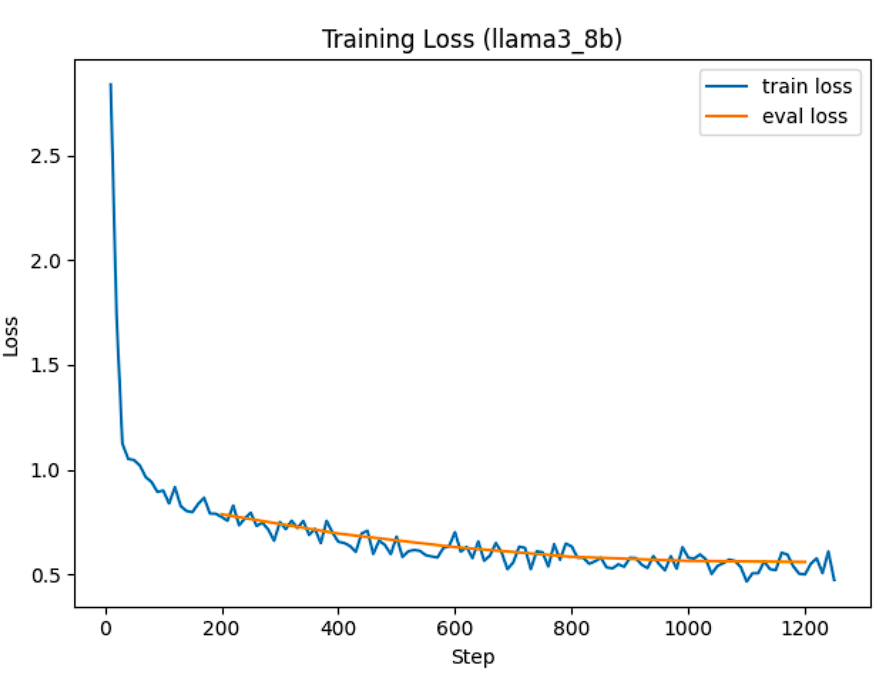
\includegraphics[width=\linewidth]{graphs/training_loss_llama8b.png}
    \caption{LLaMA3-8B}
\end{subfigure}\hfill
\begin{subfigure}[t]{0.32\textwidth}
    \centering
    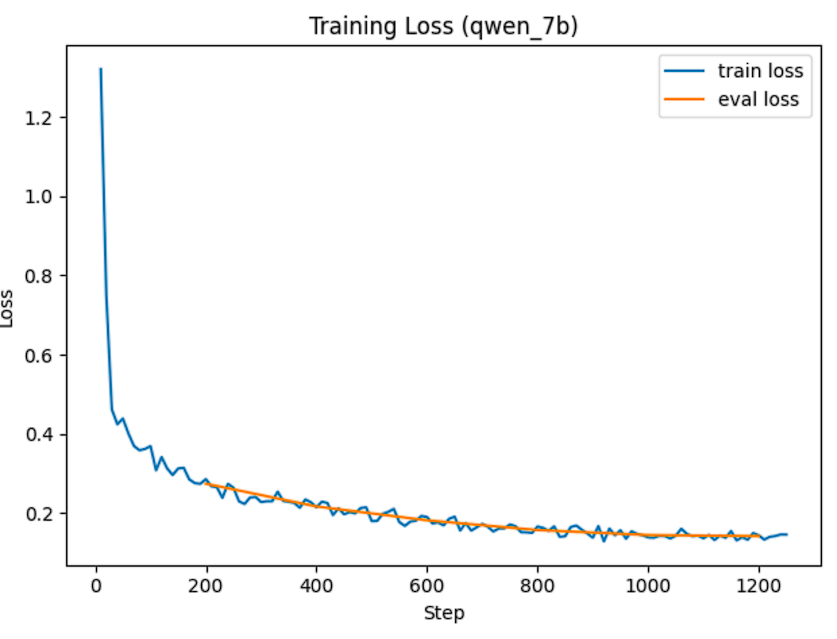
\includegraphics[width=\linewidth]{graphs/training_loss_qwen7b.png}
    \caption{Qwen2.5-7B}
\end{subfigure}\hfill
\begin{subfigure}[t]{0.32\textwidth}
    \centering
    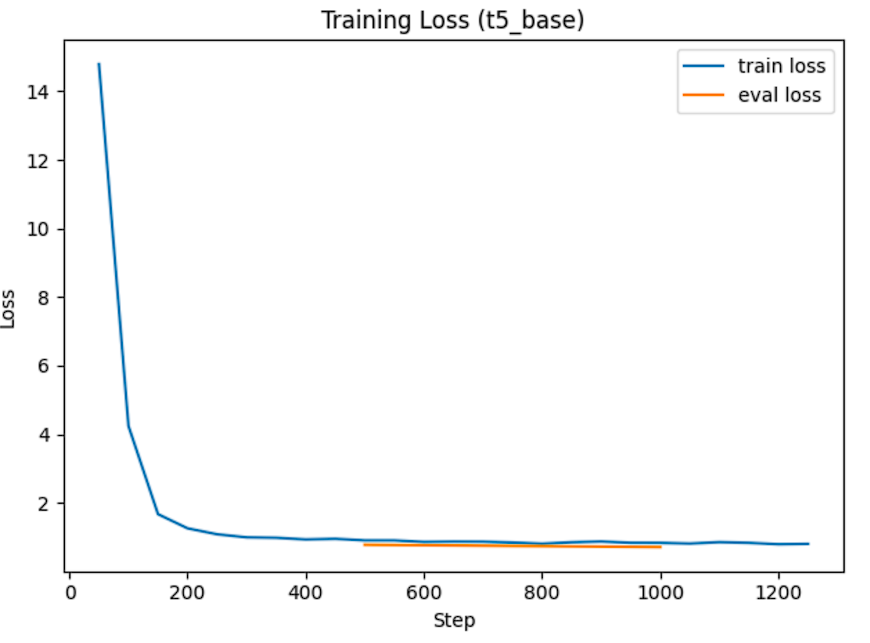
\includegraphics[width=\linewidth]{graphs/training_loss_t5base.png}
    \caption{T5-base}
\end{subfigure}

\caption{Training and evaluation loss curves during LoRA fine-tuning for representative models from different architectural families. The decoder-only models LLaMA3-8B and Qwen2.5-7B exhibit rapid and stable convergence, with training and evaluation losses decreasing consistently throughout fine-tuning. In contrast, the encoder--decoder baseline T5-base begins with substantially higher initial loss and converges more slowly. These results indicate that instruction-oriented causal language models adapt efficiently to the proposed urban-science instruction dataset under lightweight LoRA fine-tuning.}
\label{fig:training_loss}
\end{figure}
% \begin{figure}[H]
% \centering

% \begin{subfigure}{}
% \centering
% 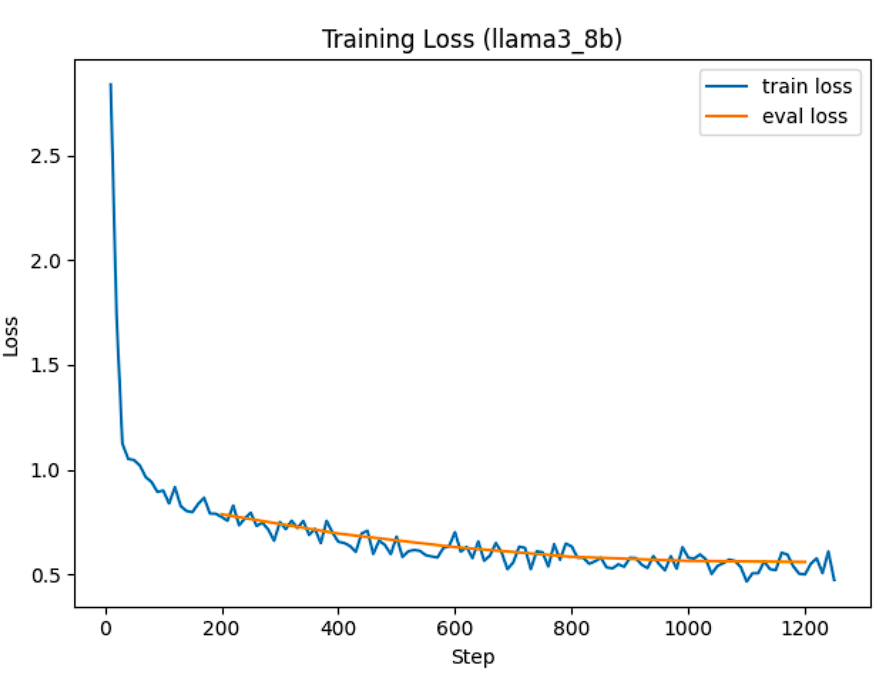
\includegraphics[width=\linewidth]{graphs/training_loss_llama8b.png}
% \caption{LLaMA3-8B}
% \end{subfigure}
% \hfill
% \begin{subfigure}{}
% \centering
% 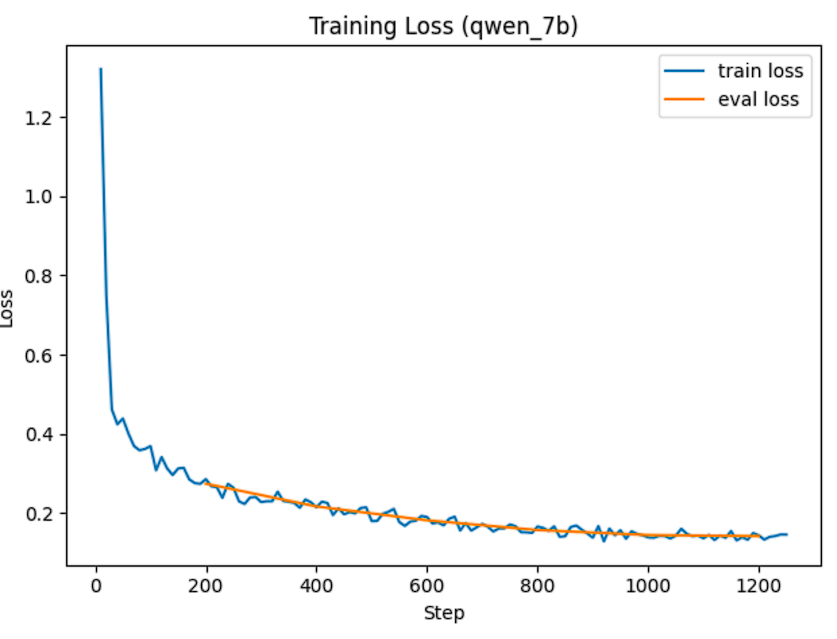
\includegraphics[width=\linewidth]{graphs/training_loss_qwen7b.png}
% \caption{Qwen2.5-7B}
% \end{subfigure}
% \hfill
% \begin{subfigure}{}
% \centering
% 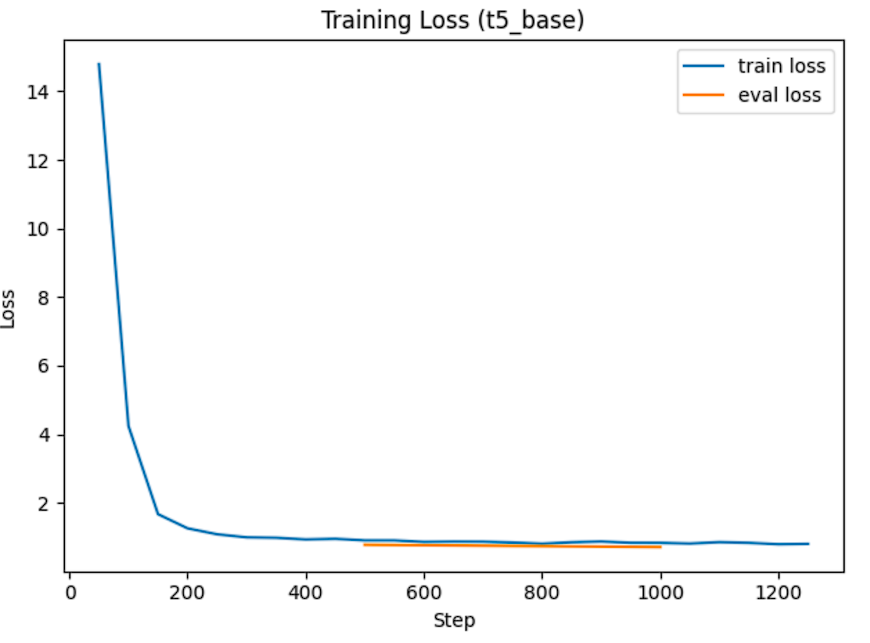
\includegraphics[width=\linewidth]{graphs/training_loss_t5base.png}
% \caption{T5-base}
% \end{subfigure}

% \caption{Training and evaluation loss curves during LoRA fine-tuning for representative models. Instruction-tuned causal language models (LLaMA and Qwen) converge rapidly and stably, while the encoder–decoder baseline T5 exhibits significantly higher initial loss and slower adaptation.}
% \label{fig:training_loss}

% \end{figure}

Figure~\ref{fig:training_loss} presents the training dynamics for three representative models: LLaMA3-8B, Qwen2.5-7B, and T5-base. These models illustrate the typical convergence behaviors observed across the different model families.

For the causal language models, both LLaMA and Qwen exhibit stable and consistent convergence. The LLaMA3-8B model shows a rapid decrease in training loss during the early training steps, dropping from approximately 2.8 to below 1.0 within the first 100 steps and gradually stabilizing near 0.55 toward the end of training. The evaluation loss closely follows the training curve, indicating stable optimization without noticeable overfitting.

The Qwen2.5-7B model demonstrates even faster convergence. Its training loss decreases sharply from approximately 1.3 to below 0.3 within the first few hundred steps and stabilizes around 0.15 in later training stages. The small gap between training and evaluation loss suggests that LoRA-based fine-tuning effectively adapts the model while maintaining generalization.

In contrast, the encoder–decoder baseline T5-base begins with a substantially higher initial loss (above 14), reflecting the difficulty of adapting a non-instruction-tuned seq2seq model to the structured instruction format of the dataset. Although the loss decreases rapidly during early training and stabilizes near 1.0, the final loss remains significantly higher than those observed for the instruction-tuned causal language models.

Overall, the training curves demonstrate stable convergence across all causal models, with Qwen models exhibiting the fastest optimization and the lowest final training loss. These results suggest that instruction-tuned causal language models are particularly well suited for adapting to structured instruction datasets through lightweight LoRA fine-tuning. Similar convergence patterns were observed for larger variants such as LLaMA3-70B and Qwen2.5-14B.

\subsection{Evaluation Performance}

We compare model performance before and after fine-tuning across multiple model families, focusing on multiple-choice answer selection, short-answer paraphrasing, and explanation generation. The evaluation highlights both improvements and degradations introduced by instruction fine-tuning.

Table~\ref{tab:eval_comparison} summarizes the performance of all models before and after fine-tuning. Overall, instruction tuning improves dataset-grounded reasoning performance, although the magnitude and characteristics of these improvements vary across model families. While Qwen models maintain their already strong baseline performance, LLaMA models exhibit substantial gains in multiple-choice accuracy, and T5-base shows notable improvements in semantic generation quality despite continuing to struggle with structured answer selection.

\begin{table}[H]
\centering
\renewcommand{\arraystretch}{1.7}
\caption{Comparison of zero-shot and post-training performance across models. \\BERTScore F1 is reported for short-answer (SA) paraphrasing.}
\label{tab:eval_comparison}
\begin{tabular}{|p{1.2cm}|p{1cm}|p{1cm}|p{1cm}|p{1cm}|p{1.5cm}|}
\hline
\textbf{Model} & \textbf{MC Acc (Pre)} & \textbf{MC Acc (Post)} & \textbf{SA BERT (Pre)} & \textbf{SA BERT (Post)} & \textbf{Trend} \\
\hline
T5-base & 0.00 & 0.00 & 0.82 & 0.90 & +Paraphrase / -Structure \\
\hline
Qwen2.5-7B & 99.97\% & 100.00\% & 0.88 & 0.90 & Stable / +Semantic Quality \\
\hline
Qwen2.5-14B & 100.00\% & 100.00\% & 0.90 & 0.91 & Stable / +Semantic Quality \\
\hline
LLaMA3-8B & 90.34\% & 95.71\% & 0.85 & 0.90 & +Accuracy / +Adaptation \\
\hline
LLaMA3-70B & 93.03\% & 97.34\% & 0.93 & 0.90 & +Accuracy / Stable Reasoning \\
\hline
\end{tabular}
\end{table}

% \begin{table}[h]
% \centering
% \caption{Comparison of zero-shot and post-training performance across models. \\BERTScore F1 is reported for short-answer (SA) paraphrasing.}
% \label{tab:eval_comparison}
% \begin{tabular}{|p{1.2cm}|p{1cm}|p{1cm}|p{1cm}|p{1cm}|p{1.5cm}|}
% \hline
% Model & MC Acc (Pre) & MC Acc (Post) & SA BERT (Pre) & SA BERT (Post) & Trend \\
% \hline
% T5-base & 0.00 & 0.00 & 0.82 & 0.90 & +Paraphrase / -Structure \\
% \hline
% Qwen2.5-7B & 99.97 & 100.00 & 0.88 & 0.85 & Stable / +Verbose \\
% \hline
% Qwen2.5-14B & 100.00 & 100.00 & 0.90 & 0.85 & Stable / ++Verbose \\
% \hline
% LLaMA3-8B & 90.34 & $23.92 & 0.85 & 0.80 & -Instruction Following / -Format Adherence \\
% \hline
% LLaMA3-70B & 93.03 & 38.59 & 0.93 & 0.83 & -Accuracy / +Overfit \\
% \hline
% \end{tabular}
% \end{table}

\begin{figure}[H]
\centering

\begin{subfigure}[t]{0.49\textwidth}
    \centering
    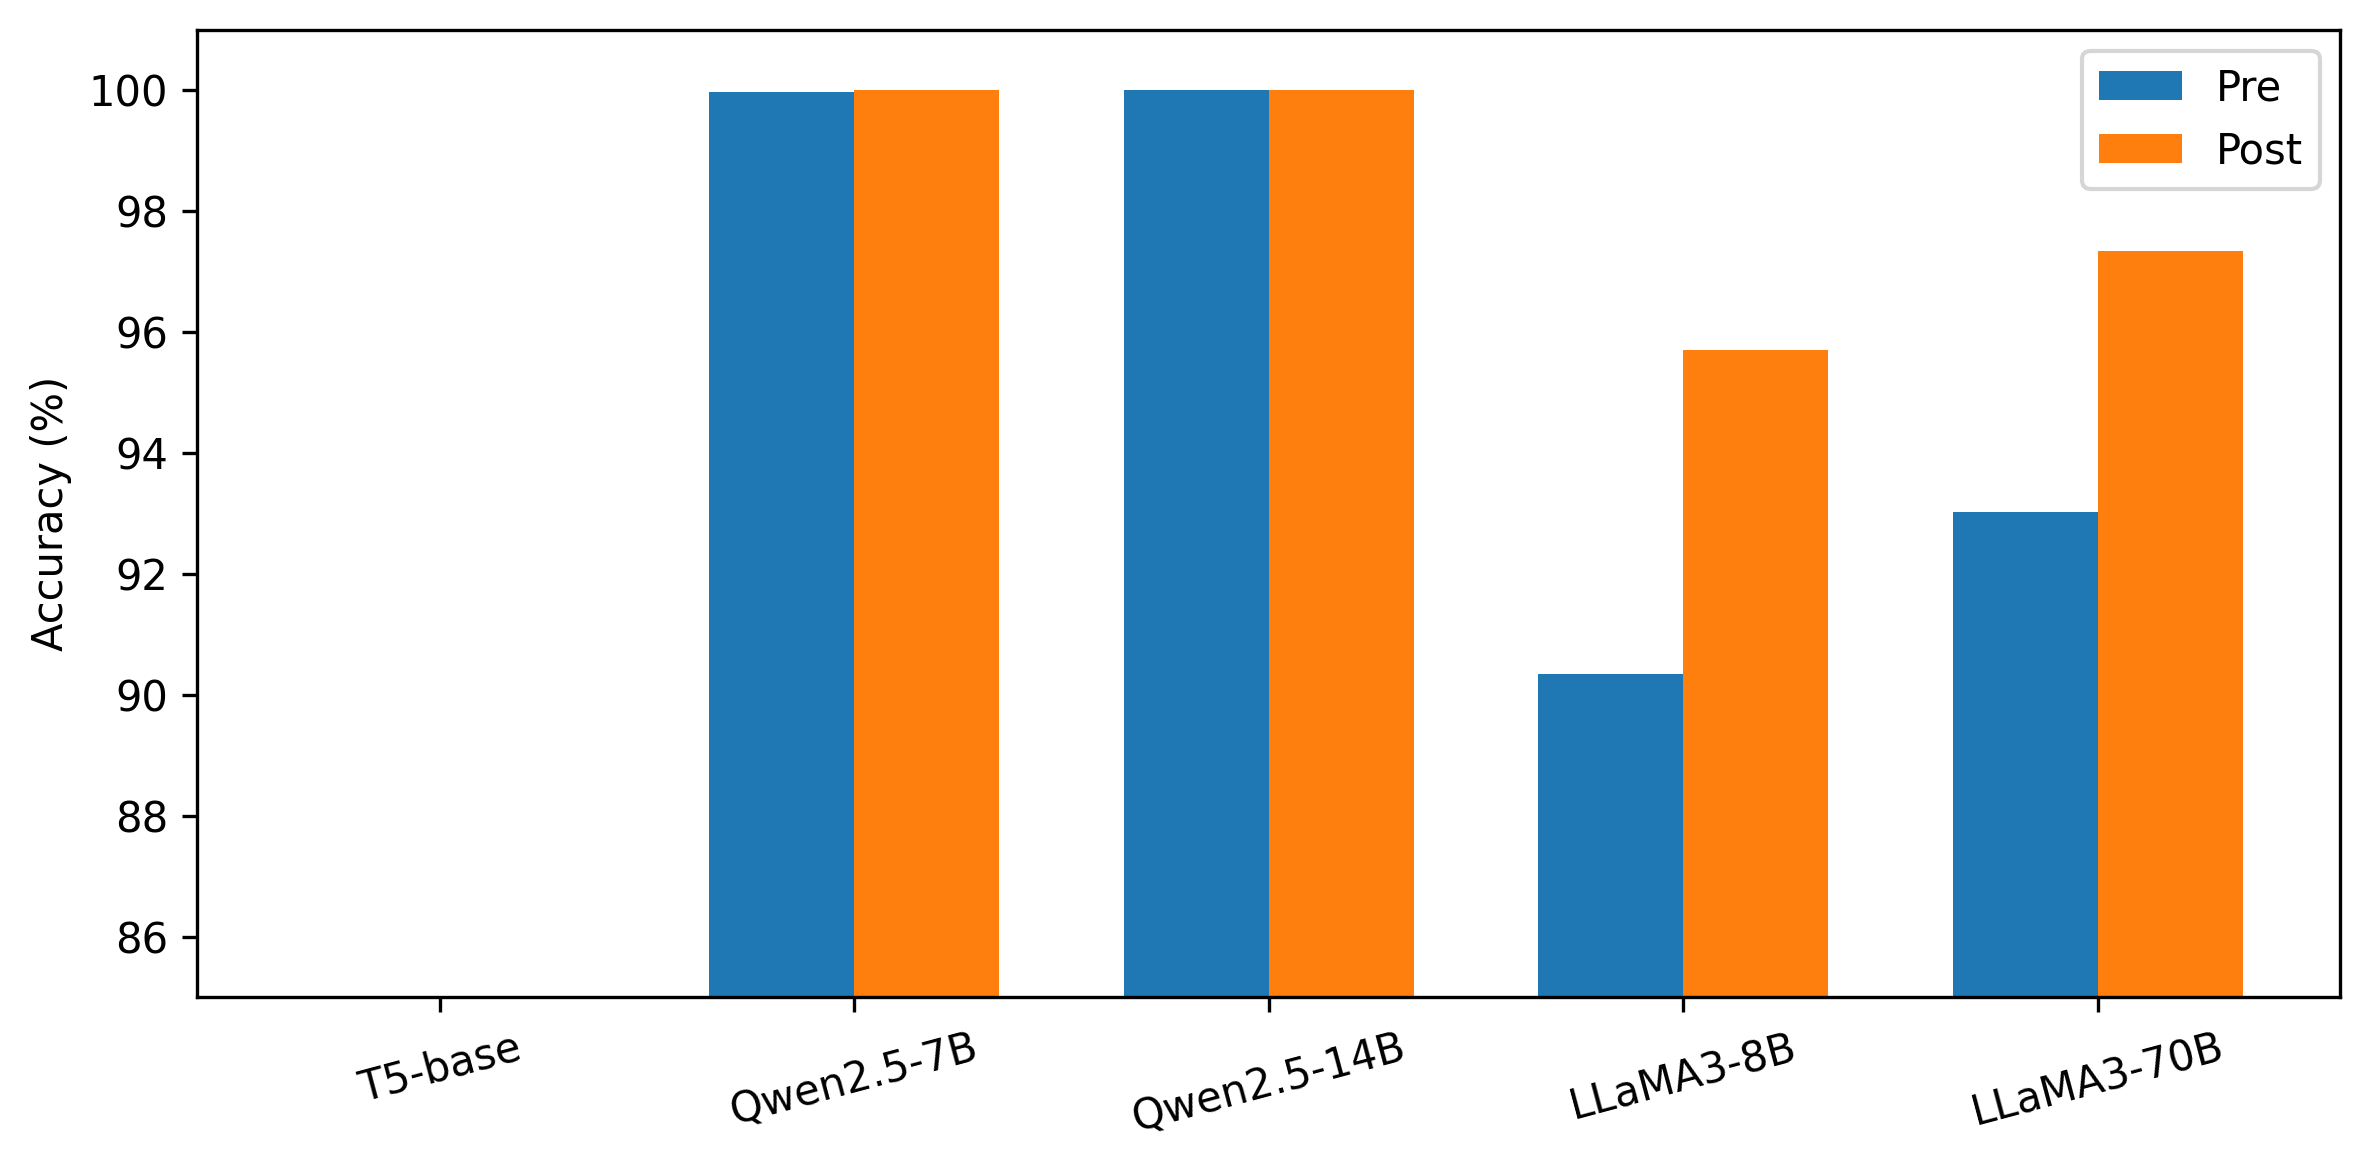
\includegraphics[width=\linewidth]{graphs/mc_accuracy_1.png}
    \caption{MC Accuracy}
    \label{fig:mc_acc}
\end{subfigure}
\hfill
\begin{subfigure}[t]{0.49\textwidth}
    \centering
    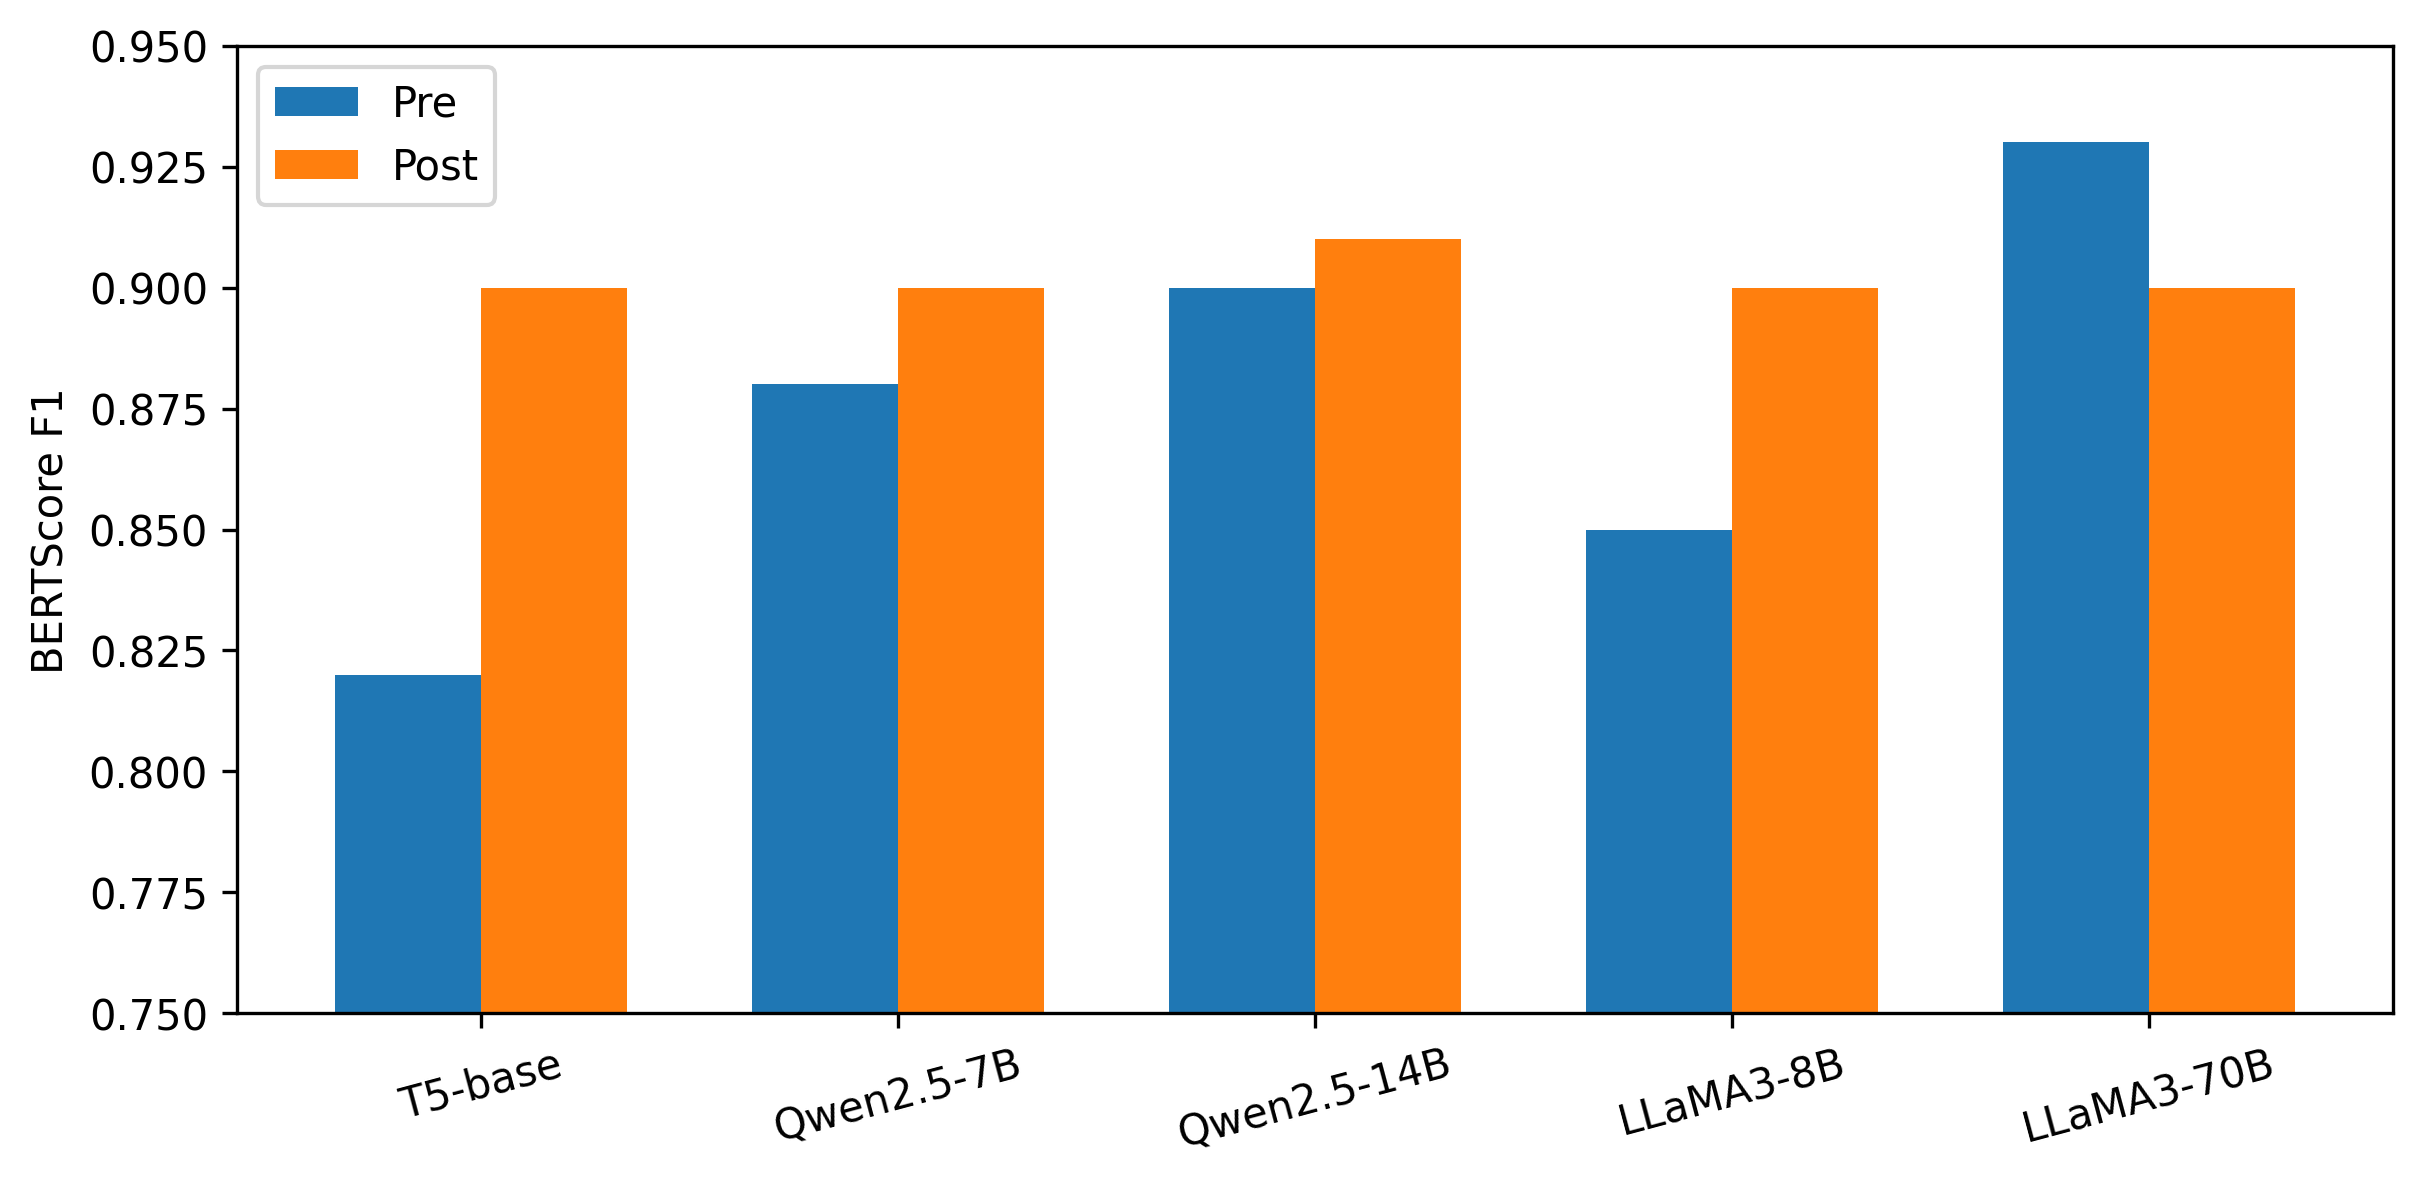
\includegraphics[width=\linewidth]{graphs/sa_bert_1.png}
    \caption{SA Paraphrasing}
    \label{fig:sa_bert}
\end{subfigure}

\caption{Comparison of pre- and post-training performance across models. Fine-tuning has heterogeneous effects across architectures. Qwen models maintain near-perfect multiple-choice accuracy, T5-base substantially improves semantic paraphrasing despite failing structured answer selection, and LLaMA3 models achieve notable gains in dataset-specific reasoning accuracy after fine-tuning.}
\label{fig:eval_perf_compare}

\end{figure}
% \begin{figure}[H]
% \centering

% \begin{subfigure}{}
% \centering
% 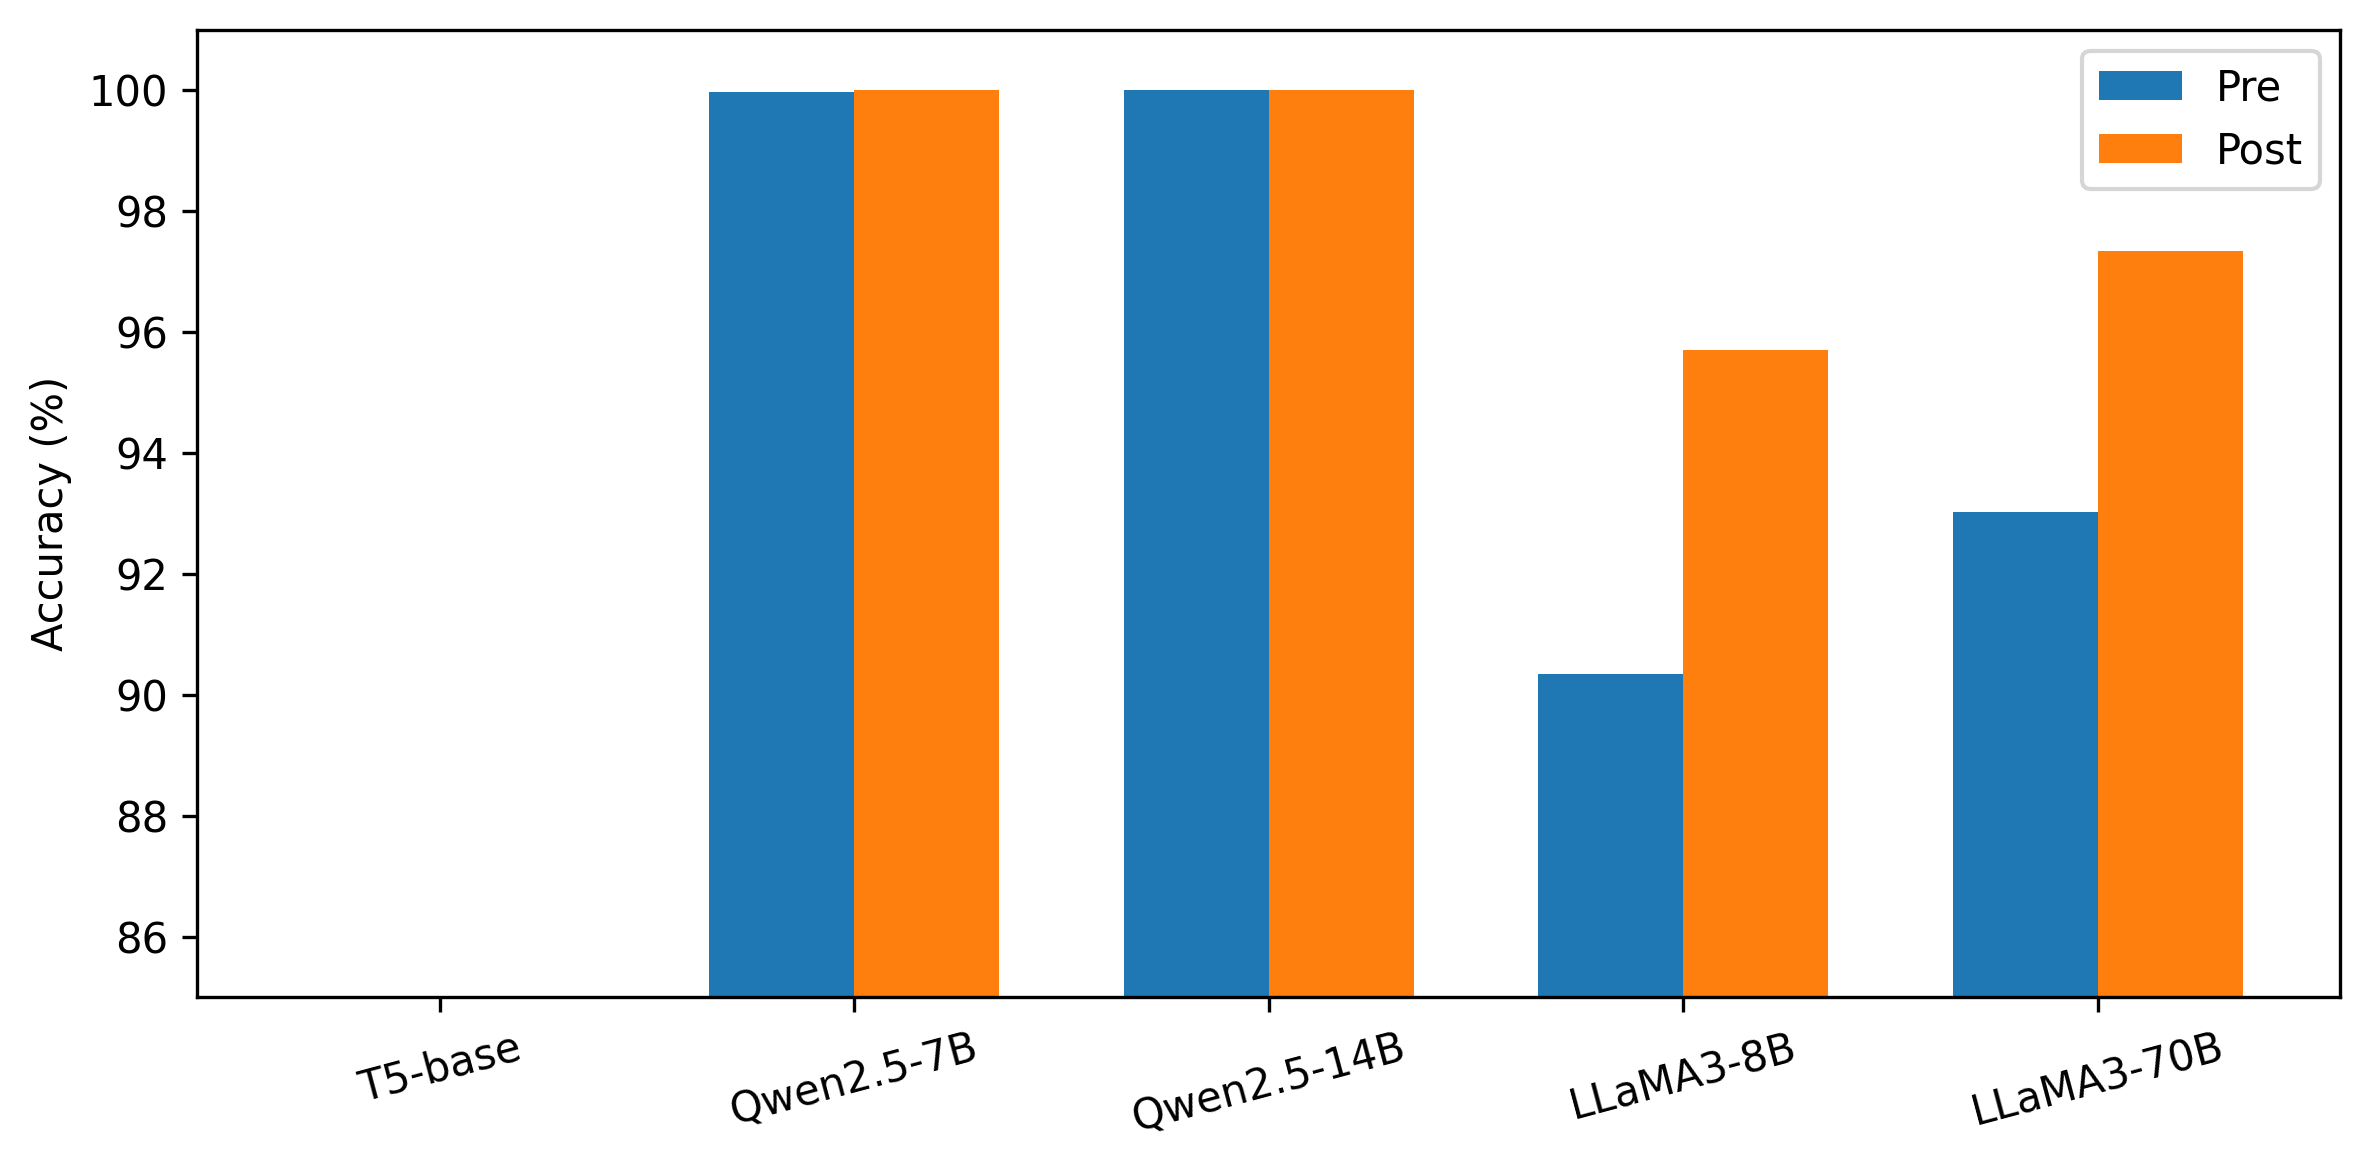
\includegraphics[width=\linewidth]{graphs/mc_accuracy_1.png}
% \caption{MC Accuracy}
% \end{subfigure}
% \hfill
% \begin{subfigure}{}
% \centering
% 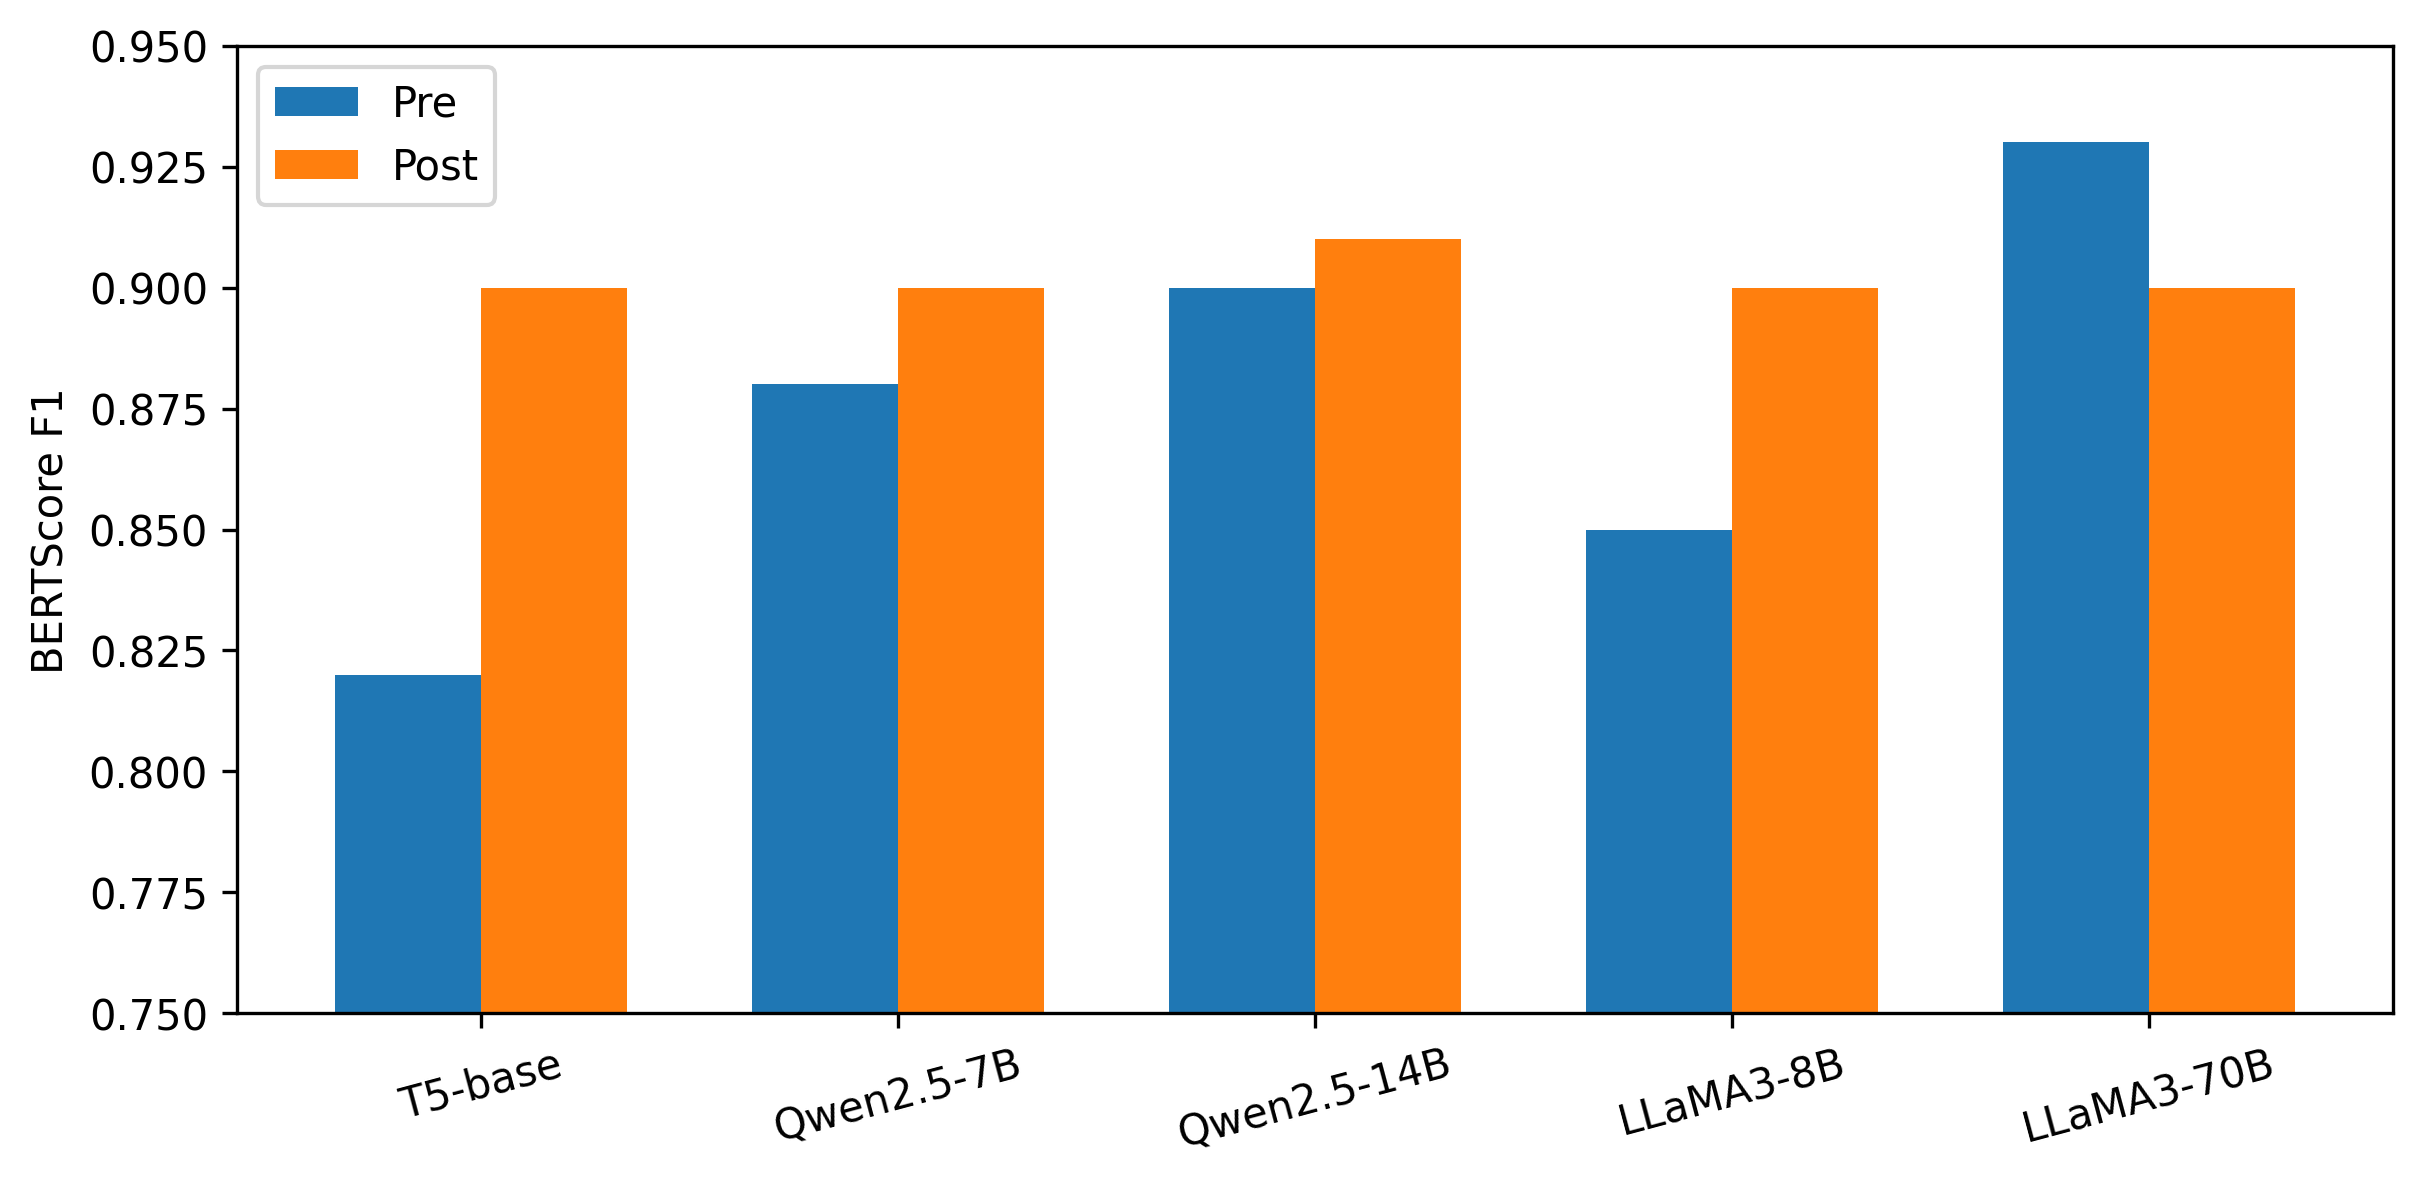
\includegraphics[width=\linewidth]{graphs/sa_bert_1.png}
% \caption{SA Paraphrasing}
% \end{subfigure}

% \caption{Comparison of pre- and post-training performance across models. Fine-tuning has heterogeneous effects across architectures. Qwen models maintain near-perfect multiple-choice accuracy, T5-base substantially improves semantic paraphrasing despite failing structured answer selection, and LLaMA3 models achieve notable gains in dataset-specific reasoning accuracy after fine-tuning.}
% \label{fig:eval_perf_compare}

% \end{figure}
The results reveal heterogeneous effects of instruction tuning across model families. Unlike the common assumption that lower training loss necessarily leads to uniform performance gains, the observed outcomes depend strongly on model architecture and task formulation.

Qwen models demonstrate the most stable behavior. Both Qwen2.5-7B and Qwen2.5-14B maintain near-perfect multiple-choice accuracy after fine-tuning, improving slightly from 99.97\% to 100.00\% and remaining at 100.00\%, respectively. Short-answer semantic similarity also improves modestly, indicating that instruction tuning reinforces existing reasoning capabilities without disrupting output quality.

The LLaMA3 models show the largest gains from instruction tuning. LLaMA3-8B improves from 90.34\% to 95.71\% multiple-choice accuracy, while LLaMA3-70B increases from 93.03\% to 97.34\%. These improvements are accompanied by higher short-answer BERTScores for LLaMA3-8B and only a slight decline for LLaMA3-70B, suggesting that fine-tuning improves dataset-specific reasoning while introducing minor trade-offs in generation style.

T5-base presents a different pattern. Although multiple-choice accuracy remains at 0\%, short-answer BERTScore improves substantially from 0.82 to 0.90. This indicates that the model benefits from exposure to domain-specific content but continues to struggle with structured answer selection tasks.

Overall, the results suggest that instruction tuning is generally beneficial for dataset-grounded urban reasoning, particularly for decoder-only language models. However, the magnitude and nature of the gains vary substantially across architectures.

\subsection{Performance by Model Family and Scale}

\paragraph{Per-Model Comparison}

Across models, fine-tuning produces substantially different effects depending on architecture and scale.

\textbf{LLaMA3 Models.}
Both LLaMA3 models benefit substantially from instruction tuning. LLaMA3-8B improves from 90.34\% to 95.71\% multiple-choice accuracy, while LLaMA3-70B improves from 93.03\% to 97.34\%. These gains indicate that the proposed instruction dataset successfully teaches domain-specific dataset interpretation and improves answer selection accuracy.

While the models occasionally generate longer responses and additional explanatory content, they retain strong instruction-following behavior and demonstrate improved performance on structured reasoning tasks. The larger LLaMA3-70B model achieves the strongest post-training classification performance among the LLaMA variants, suggesting that increased model capacity can effectively leverage the dataset-specific supervision provided during fine-tuning.

\textbf{Qwen Models.}
Both Qwen2.5-7B and Qwen2.5-14B maintain perfect multiple-choice accuracy (100\%) after fine-tuning, indicating strong robustness in constrained classification tasks. 

However, both models exhibit increased verbosity in generative tasks. Qwen2.5-7B tends to produce structured outputs that include additional sections such as ``Answer,'' ``Explanation,'' and ``Note,'' while Qwen2.5-14B further amplifies this behavior by generating extended meta-commentary and self-reflective text. Despite this verbosity, semantic similarity remains relatively stable, with BERTScore values around 0.85, suggesting that the core content is preserved even as output structure becomes more elaborate.

\textbf{T5-base.}
T5-base continues to fail on multiple-choice answer selection after fine-tuning, with 0\% accuracy across all settings. In contrast, its paraphrasing performance improves substantially, achieving a BERTScore of 0.90. However, the model frequently produces malformed outputs that repeat instruction blocks or omit required answer components, indicating poor adherence to structured output constraints despite improved semantic generation.

\paragraph{Zero-Shot vs Fine-Tuned Performance}

Comparing zero-shot and fine-tuned performance reveals that instruction tuning generally improves model behavior, although the magnitude of improvement differs across architectures.

Qwen models remain highly stable, preserving near-perfect multiple-choice accuracy while slightly improving semantic similarity. This suggests that strong instruction-following capabilities acquired during pretraining can be reinforced without sacrificing robustness.

LLaMA models experience the largest gains from fine-tuning. Both model sizes show improvements of more than four percentage points in classification accuracy, indicating that the proposed dataset effectively transfers urban-science reasoning patterns to previously unseen tasks.

T5-base exhibits improved semantic generation quality but continues to struggle with constrained classification outputs. This suggests that encoder-decoder architectures may benefit from alternative task formulations that better align with their generative training objectives.

Overall, instruction tuning improves dataset-grounded reasoning performance for decoder-only architectures while primarily enhancing semantic generation quality for encoder-decoder models.

\paragraph{Cross-Model Comparison}

Across architectures, distinct patterns emerge:

\begin{itemize}
    \item \textbf{Causal LLMs (LLaMA, Qwen)} achieve strong multiple-choice reasoning performance in both zero-shot and fine-tuned settings.
    
    \item \textbf{Qwen models} demonstrate the greatest robustness, maintaining near-perfect accuracy while slightly improving semantic similarity.
    
    \item \textbf{LLaMA models} benefit substantially from instruction tuning, showing notable gains in classification accuracy and improved urban-science reasoning performance.
    
    \item \textbf{Encoder--decoder models (T5)} improve semantic paraphrasing quality but remain ineffective for constrained answer-selection tasks.
\end{itemize}

These findings suggest that model architecture plays a critical role in determining how instruction tuning affects both reasoning performance and output behavior.

\paragraph{Key Findings}

From the combined evaluation, several key findings emerge:

\begin{itemize}
    \item Fine-tuning generally improves dataset-grounded reasoning performance for decoder-only language models.
    
    \item Architectural differences strongly influence how models respond to instruction tuning.
    
    \item Qwen models exhibit the most stable behavior, maintaining near-perfect performance before and after fine-tuning.
    
    \item LLaMA models achieve the largest relative gains, suggesting that domain-specific instruction tuning effectively improves structured urban-science reasoning.
    
    \item Improvements in semantic similarity do not always correspond to improvements in structured answer selection, as illustrated by T5-base.
    
    \item Strong zero-shot performance provides a useful foundation, but instruction tuning can still yield measurable gains on specialized urban-science tasks.
\end{itemize}

Overall, the evaluation highlights that instruction fine-tuning on dataset-centric tasks introduces complex trade-offs between semantic correctness, structural fidelity, and task compliance, rather than uniformly improving model performance.

\subsection{Performance by Task Type and Difficulty Level}

We analyze model performance across task types—multiple-choice (MC) and short-answer (SA)—as well as across different difficulty levels (Level~1 to Level~3). This analysis provides insight into how models handle structured reasoning under varying levels of complexity.

\paragraph{Performance by Task Type}

A clear distinction emerges between multiple-choice and short-answer tasks. 

For multiple-choice answer selection, causal language models (LLaMA and Qwen) demonstrate strong zero-shot performance, with near-perfect accuracy for Qwen models and high accuracy for LLaMA models. After fine-tuning, Qwen models maintain perfect performance, while both LLaMA3 models achieve substantial improvements in multiple-choice accuracy, demonstrating effective adaptation to the dataset-specific reasoning tasks. In contrast, T5-base consistently fails on multiple-choice tasks, both before and after fine-tuning, indicating difficulty in producing constrained outputs.

For short-answer paraphrasing, all models achieve relatively high semantic similarity scores as measured by BERTScore. T5-base achieves the highest post-training performance, indicating strong capability in generating semantically faithful text. Qwen models maintain stable paraphrasing quality with moderate decreases after fine-tuning, while LLaMA models show lower and less stable performance, particularly for smaller-scale variants.

These results highlight a fundamental trade-off: models that perform well on constrained classification tasks do not necessarily produce high-quality structured generation, and vice versa.

\paragraph{Performance by Difficulty Level}

Across difficulty levels, several consistent trends are observed. For short-answer paraphrasing, performance generally improves with increasing task complexity. Higher BERTScore values are observed for Level~2 and Level~3 tasks compared to Level~1, particularly for T5-base and Qwen models. This may be attributed to longer or more descriptive target outputs in higher-level tasks, which provide more context for semantic matching.

For multiple-choice tasks, Qwen models maintain stable performance across levels, indicating robustness to increasing reasoning complexity. Similarly, LLaMA3-70B demonstrates improved performance across both Level~1 and Level~2 tasks after fine-tuning, suggesting that the proposed instruction dataset effectively enhances structured urban-science reasoning across different levels of task complexity.

\paragraph{Interaction Between Task Type and Difficulty}

The interaction between task type and difficulty further highlights differences in model behavior. While higher-level tasks tend to improve paraphrasing scores, they do not necessarily improve structured output compliance. Models such as Qwen2.5-14B and T5-base often generate more verbose or structured responses for higher-level tasks, which can introduce redundancy or formatting inconsistencies.

Overall, these findings suggest that increasing task difficulty does not uniformly challenge models in the same way across task types. Instead, task formulation—whether requiring constrained selection or open-ended generation—plays a more significant role in determining model performance than difficulty level alone.

\subsection{Cross-Regional Generalization Results}

To evaluate the transferability of dataset-centric reasoning, we assess model performance on cross-regional test sets constructed from the \textit{Île-de-France Mobilités Open Data} dataset~\cite{idfm2024} (France) and the \textit{MLIT Traffic Census} dataset~\cite{mlit2024} (Japan). These datasets differ from the training sources in naming conventions, schema design, and contextual semantics, providing realistic benchmarks for evaluating generalization beyond the original domain.

The Île-de-France Mobilités dataset is released by the regional transportation authority in Paris, while the MLIT dataset is provided by Japan’s Ministry of Land, Infrastructure, Transport and Tourism. Together, they represent diverse geographic, linguistic, and structural variations in urban transportation data.

\subsubsection{Overall Performance Trends}

The results reveal substantial variation across model families and scales. Qwen-based models demonstrate the strongest cross-regional performance, with Qwen2.5-7B achieving 100\% accuracy and Qwen2.5-14B achieving 98\%. LLaMA3 models also generalize effectively, with LLaMA3-70B achieving 98\% accuracy and LLaMA3-8B achieving 97\%, indicating that dataset-centric reasoning transfers well across regions for decoder-only architectures. In contrast, T5-base achieves 0\% accuracy on the multiple-choice task, highlighting persistent difficulties with constrained answer-selection despite fine-tuning.

Despite these differences in classification performance, most models maintain moderate to high semantic similarity in generative tasks. BERTScore F1 values remain above 0.75 across all models, indicating that even models with weaker structured-output performance retain substantial understanding of the underlying dataset semantics.

\subsubsection{Model Family Behavior}

The results highlight distinct behaviors across model architectures.

\textbf{T5-base.}
T5-base fails entirely on the multiple-choice task due to its sequence-to-sequence formulation, which does not align with constrained classification objectives. Instead of selecting a single option (e.g., ``B''), the model generates full-text responses that restate the correct answer. However, it achieves strong performance on paraphrasing tasks (BERTScore $\sim$0.86), indicating robust semantic transformation capabilities.

\textbf{LLaMA3 Models.}
Both LLaMA3 models demonstrate strong cross-regional generalization. LLaMA3-8B achieves approximately 97\% multiple-choice accuracy, while LLaMA3-70B reaches approximately 98\%, indicating that the learned dataset-centric reasoning patterns transfer effectively to unseen regional datasets. In generative tasks, both models maintain moderate to high semantic similarity, with BERTScore values ranging from approximately 0.80 to 0.85. Although the models occasionally generate longer responses than required, overall performance remains stable across both classification and paraphrasing evaluations.

\textbf{Qwen Models.}
Both Qwen2.5-7B and Qwen2.5-14B demonstrate the strongest cross-regional generalization, maintaining near-perfect accuracy on unseen datasets. Qwen2.5-7B exhibits the most stable behavior with consistent formatting and controlled outputs, while Qwen2.5-14B achieves comparable accuracy but occasionally produces more verbose assistant-style responses. Overall, the Qwen family demonstrates the highest level of robustness under regional distribution shifts.

\subsubsection{Paraphrase Performance}

Across all models, paraphrasing performance remains relatively stable in terms of semantic similarity, as reflected by BERTScore F1 values ranging from approximately 0.78 to 0.86. However, lexical overlap (ROUGE) varies significantly. T5-base achieves the highest ROUGE scores (up to $\sim$0.43), while LLaMA3 models exhibit substantially lower scores ($\sim$0.07–0.17), reflecting structural instability. Qwen models achieve moderate ROUGE scores ($\sim$0.16–0.23), indicating a balance between semantic preservation and structural consistency.

Overall, the results show that while semantic understanding transfers across regions, model performance is highly sensitive to output constraints and instruction-following behavior. Qwen-based models achieve the most robust cross-regional performance, while other models exhibit varying degrees of degradation due to format non-compliance and generation instability.

\subsection{Dataset-Centric Findings and Analysis}

Beyond quantitative evaluation, we analyze model behavior to understand how the structure and design of the instruction dataset influence learning outcomes. Our findings reveal several consistent patterns across model families and cross-regional settings.

\paragraph{Semantic Transfer and Task Adaptation}

A central observation is that instruction tuning successfully transfers dataset-specific reasoning knowledge across multiple architectures. Models that already possess strong zero-shot capabilities, particularly Qwen and LLaMA, further improve after exposure to the proposed urban-science instruction dataset.

This indicates that cross-regional generalization is not limited by knowledge transfer, but rather by the ability to conform to task-specific output formats.

\paragraph{Instruction Alignment as a Key Factor}

Models with stronger instruction-following capabilities exhibit the most stable adaptation behavior. Qwen models maintain nearly perfect performance both before and after fine-tuning, suggesting that alignment and domain adaptation can complement one another rather than compete.

\paragraph{Scaling and Adaptability}

Larger models generally achieve stronger overall performance, although the gains are not strictly proportional to model size. While Qwen2.5-14B achieves the highest overall semantic quality, LLaMA3-8B demonstrates that relatively smaller models can still benefit substantially from domain-specific supervision.

\paragraph{Format Overfitting}

Models tend to overfit to the structural format of the instruction data. Instead of producing minimal task-compliant outputs, they frequently reproduce full instruction templates, including fields such as `Fact,'' `Question,'' and ``Explanation.'' This behavior is particularly pronounced in causal language models, where outputs often mirror the input structure.

\paragraph{Verbosity and Overgeneration}

Instruction fine-tuning consistently increases output verbosity. Models often append unnecessary explanations, meta-level commentary, or conversational elements (e.g., ``Note'' sections). Larger models amplify this effect, producing extended outputs that deviate from the intended concise format.

\paragraph{Task Misalignment and Output Drift}

Fine-tuning can introduce task misalignment, where models deviate from strict output requirements. For example, LLaMA3-70B frequently generates correct answers in extended form (e.g., ``The best answer is B'') rather than the required format, leading to evaluation failure despite correct reasoning.

\paragraph{Repetition and Degeneration}

Some models exhibit repetition and degeneration in generated text, including duplicated phrases and recursive expansions. This suggests instability in generation, particularly when models are fine-tuned on highly structured instruction data without explicit constraints on output length or format.

\paragraph{Impact of Dataset Design}

These behaviors can be traced to characteristics of the dataset design. The use of consistent structured formats and detailed explanations encourages models to learn both reasoning and formatting patterns. However, without explicit penalties for verbosity or format deviation, models may prioritize reproducing structure over producing minimal, task-compliant outputs.

\paragraph{Summary of Findings}

Overall, our analysis reveals that instruction fine-tuning on structured, dataset-centric tasks introduces systematic behavioral shifts:

\begin{itemize}
\item Semantic understanding transfers well, but structural compliance remains fragile.
\item Instruction alignment is essential for robust generalization.
\item Scaling introduces a trade-off between reasoning ability and output control.
\item Models exhibit format overfitting, verbosity, and occasional generation instability.
\end{itemize}

These findings emphasize that dataset design and training objectives must carefully balance reasoning, structure, and output control to achieve reliable performance across domains.


% \section{Result}\label{sec5}
% \subsection{Training loss} 

% The training loss graphs for Llama3, BERT, and T5 demonstrate the convergence patterns for each model during fine-tuning.

% \textit{Llama3:}(Figure~\ref{fig:llama3_loss}) The training loss decreases steadily, reflecting effective optimization.

% \textit{BERT:}(Figure~\ref{fig:bert_loss}) The training loss exhibits a gradual decline with some fluctuations, typical for large-scale fine-tuning.

% \textit{T5:}(Figure~\ref{fig:t5_loss}) The loss rapidly decreases and stabilizes, showcasing efficient learning during training.

% \begin{figure}[h!]
%     \centering
%     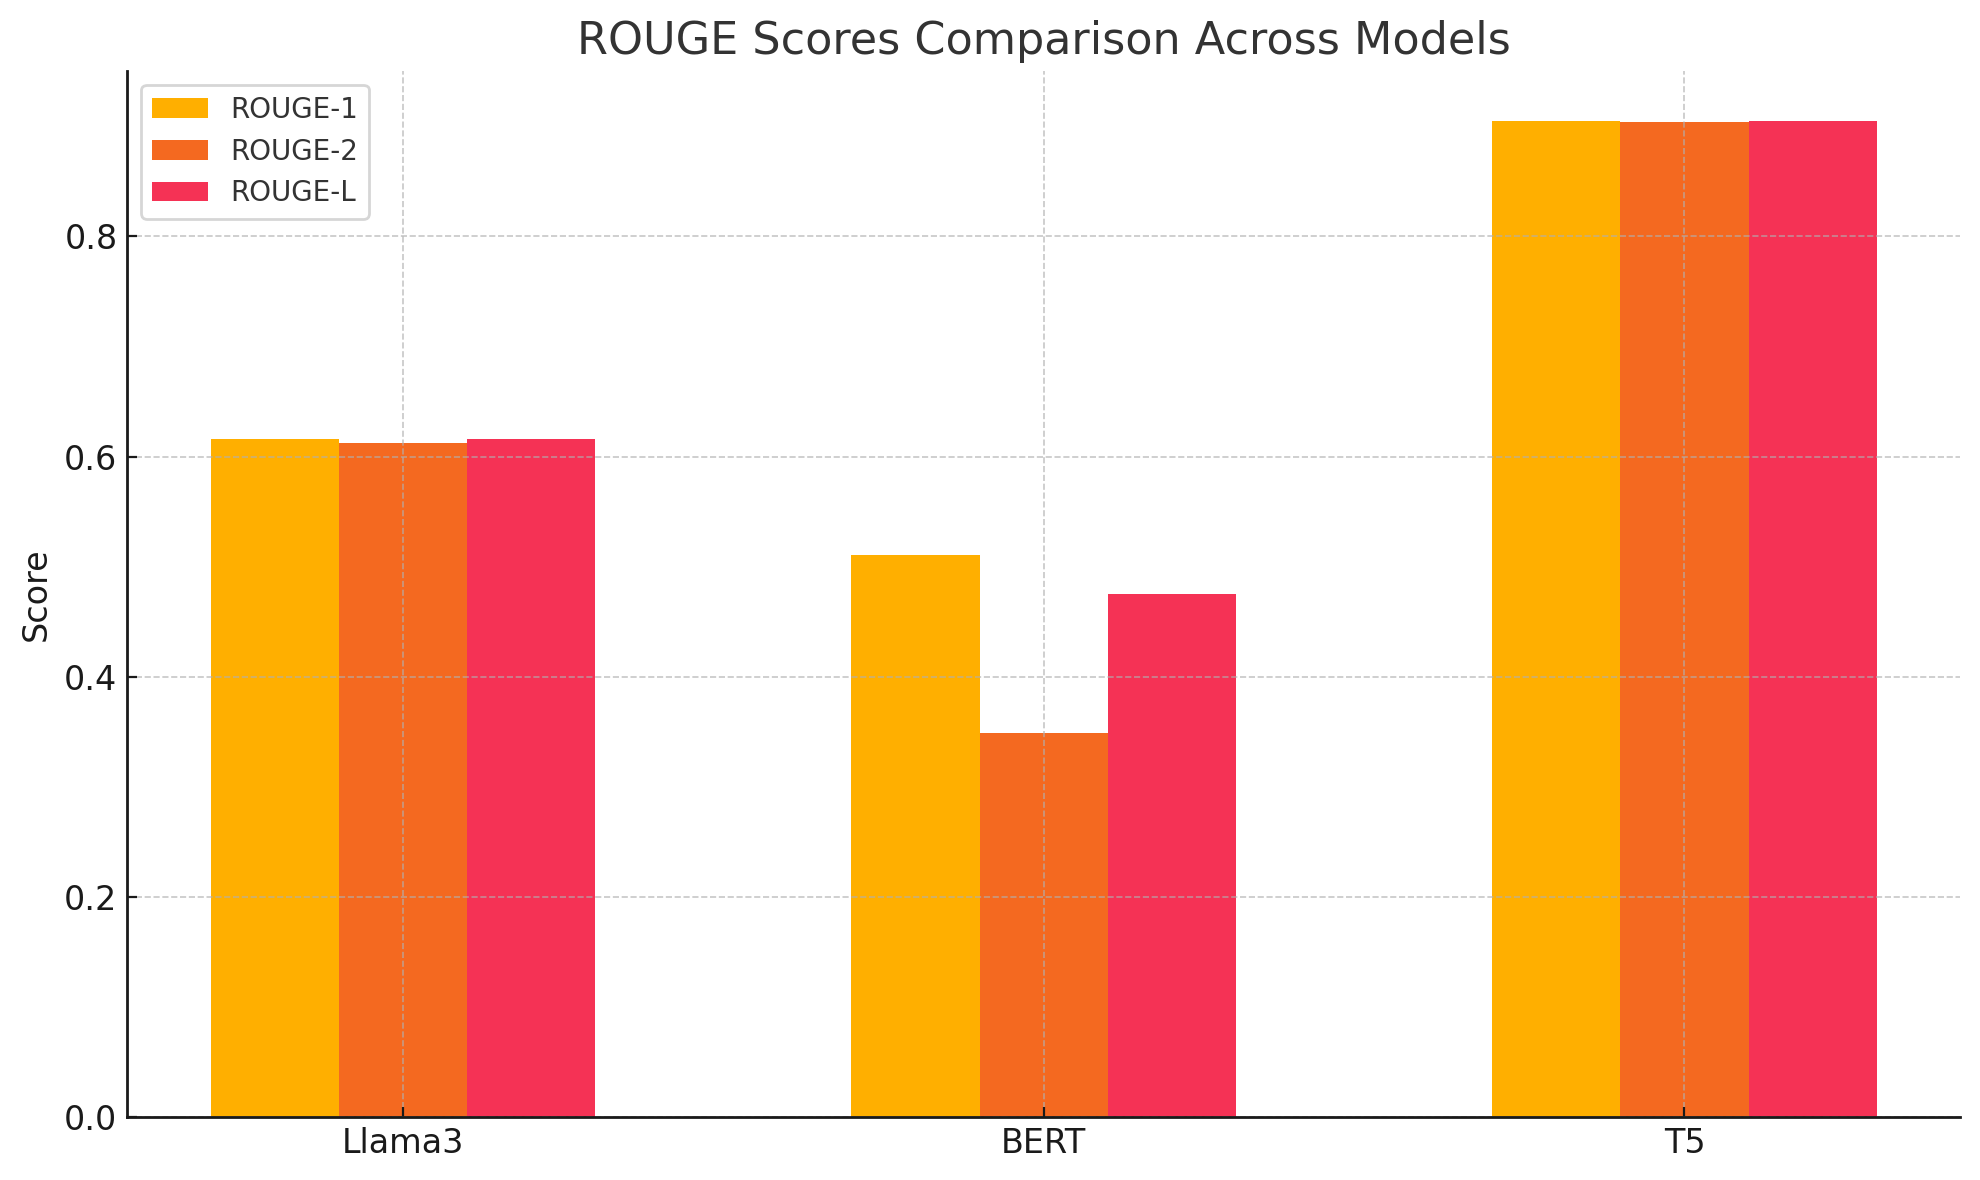
\includegraphics[width=0.4\textwidth]{./plots/llama3_training_loss.jpg}
%     \caption{Training Loss for Llama3}
%     \label{fig:llama3_loss}
% \end{figure}

% \begin{figure}[h!]
%     \centering
%     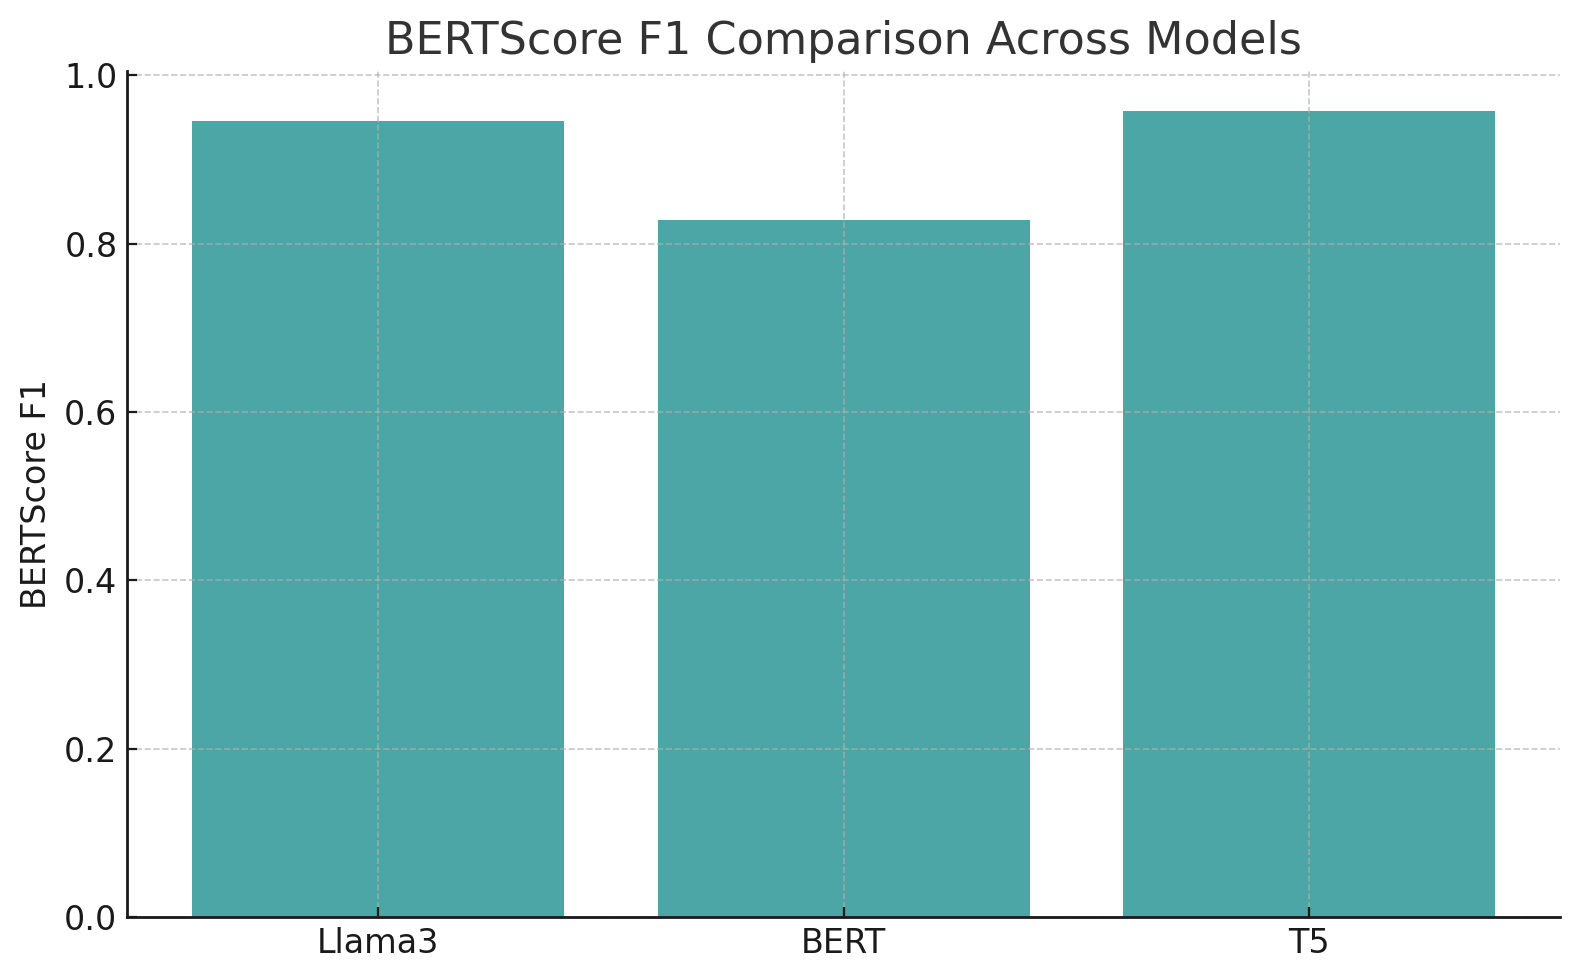
\includegraphics[width=0.4\textwidth]{./plots/bert_training_loss.png}
%     \caption{Training Loss for BERT}
%     \label{fig:bert_loss}
% \end{figure}

% \begin{figure}[h!]
%     \centering
%     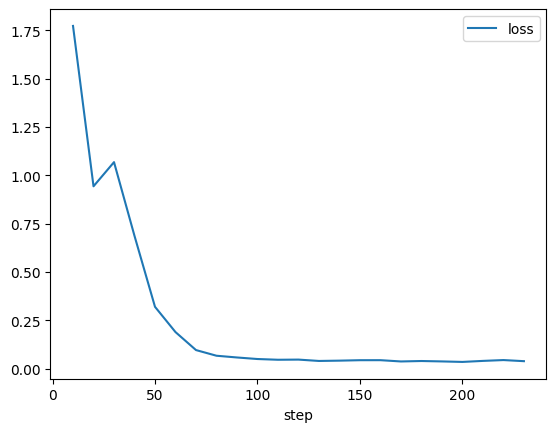
\includegraphics[width=0.4\textwidth]{./plots/t5_training_loss.png}
%     \caption{Training Loss for T5}
%     \label{fig:t5_loss}
% \end{figure}

% \subsection{Evaluation Metrics}

% \begin{figure}[h!]
%     \centering
%     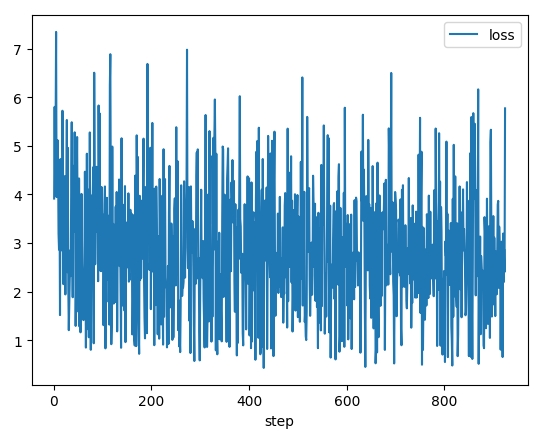
\includegraphics[width=0.4\textwidth]{./plots/bertscore.png}
%     \caption{BERTScore F1 Comparison Across Models}
%     \label{fig:bertscore}
% \end{figure}


% The BERTScore F1 (Figure~\ref{fig:bertscore}) metric evaluates semantic similarity between model outputs and reference responses:

% \begin{itemize}
%     \item \textbf{Llama3}: Achieved a high BERTScore F1 of 0.928, reflecting strong semantic alignment.
%     \item \textbf{BERT}: Scored 0.875, indicating lower performance in preserving semantic meaning.
%     \item \textbf{T5}: Achieved the highest BERTScore F1 of 0.954, confirming its superior ability to generate semantically accurate responses.
% \end{itemize}

% \begin{figure}[h!]
%     \centering
%     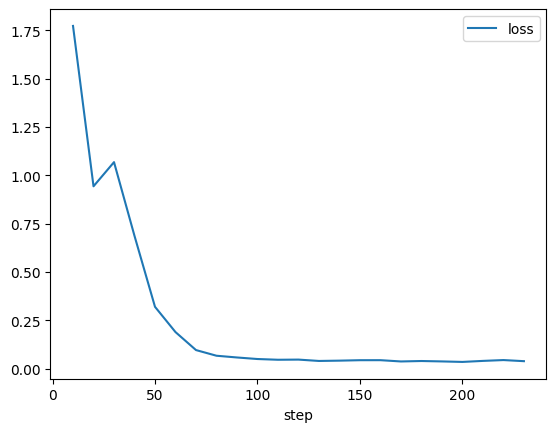
\includegraphics[width=0.4\textwidth]{./plots/rouguescore.png}
%     \caption{Rouge Score Comparison Across Models}
%     \label{fig:roguescore}
% \end{figure}

% The comparison of ROUGE scores (Figure~\ref{fig:roguescore}) across models highlights their performance in generating responses:

% \begin{itemize}
%     \item \textbf{Llama3}: Achieved ROUGE-1, ROUGE-2, and ROUGE-L scores of 0.668, 0.665, and 0.669, respectively, showing strong consistency in text overlap with reference responses.
%     \item \textbf{BERT}: Achieved lower ROUGE scores (ROUGE-1: 0.425, ROUGE-2: 0.277, ROUGE-L: 0.384), indicating moderate alignment with the references.
%     \item \textbf{T5}: Significantly outperformed the other models with ROUGE-1, ROUGE-2, and ROUGE-L scores over 0.89, indicating superior generation quality.
% \end{itemize}

% \subsection{Cross-Regional Generalization Results}

% To assess how well each model generalizes to unseen geographical data, we evaluated them on the instruction datasets from France and Japan. The performance, measured in a zero-shot setting, is summarized in Table~\ref{tab:cross_regional_results}.

% \begin{table}[h!]
% \centering
% \caption{Cross-Regional Generalization Performance on Unseen Datasets}
% \label{tab:cross_regional_results}
% \resizebox{\columnwidth}{!}{%
% \begin{tabular}{|p{3.5cm}|p{1.8cm}|p{1.5cm}|p{1.5cm}|p{1.5cm}|}
% \hline
% \textbf{Model} & \textbf{BERTScore F1} & \textbf{ROUGE-1} & \textbf{ROUGE-2} & \textbf{ROUGE-L} \\ \hline
% Llama-3.1-8B    & 0.928                 & 0.540            & 0.536            & 0.540            \\ \hline
% google-bert/bert-base-cased & 0.795     & 0.781            & 0.553            & 0.728            \\ \hline
% t5-base         & \textbf{0.957}        & \textbf{0.948}   & \textbf{0.942}   & \textbf{0.949}   \\ \hline
% \end{tabular}%
% }
% \end{table}

% The results in the table confirm that T5 generalizes most effectively to the unseen regional datasets, maintaining exceptionally high scores across all metrics. Llama3 also retains considerable robustness, showing strong semantic alignment with a high BERTScore. BERT, though still capable, exhibited a more noticeable decline in performance, particularly in its BERTScore F1. 

% Overall, these findings indicate that our instruction dataset helps LLMs develop transferable knowledge for international urban planning contexts, even without region-specific fine-tuning.


% \section{Analysis}\label{sec6}
% In this study, we evaluated the performance of fine-tuned models on an instruction dataset specifically designed for urban planning tasks. Our analysis focused on 20 selected examples generated by each model, with particular attention to cases where the BERTS score F1 was high but the ROUGE score was low. These highlighted cases where the model's outputs exhibit strong semantic similarity to the reference responses but limited textual overlap. The conclusions drawn from this analysis are as follows.

% \subsection{Model Performance Analysis}

% \begin{itemize}
%     \item \textbf{Llama3}: The primary issue with Llama3 lies in its tendency to generate excessively lengthy and verbose explanations within the "reason" section. These overly elaborate responses often fail to address the core content of the question or provide a clear connection to the true explanation. Instead, the additional verbosity introduces misleading or irrelevant information, which detracts from the clarity and precision of the intended reasoning. While the actual explanation is typically present somewhere within the generated text, it is often buried within the excessive details and unrelated content. This makes it challenging to identify and extract the true intent of the response, ultimately impacting the model's ability to produce concise, accurate, and contextually aligned explanations.

%     \item \textbf{T5}: The results produced by T5 demonstrate a high degree of alignment with the original intent of the dataset, largely due to the incorporation of the "paraphrase" keyword during training. This training approach enables the model to effectively capture the nuances and requirements of the dataset, leading to consistently high performance as reflected in both BERT and ROUGE scores. Even in instances where ROUGE-L scores are slightly lower, the deviations can typically be attributed to minor formatting inconsistencies or occasional repetition within the "reason" section. These discrepancies, however, are largely superficial and do not significantly impact the overall quality or accuracy of the generated responses. T5’s ability to maintain fidelity to the dataset's intent while delivering robust and well-structured outputs underlines its effectiveness as a model for instruction-heavy tasks.

%     \item \textbf{BERT}: The results generated by BERT reveal significant issues, as the outputs frequently consist of incoherent or nonsensical content. While there are instances where the model achieves non-negligible BERTScores, these scores do not reflect the quality or interpretability of the generated responses. The content often lacks clarity and fails to convey any meaningful or relevant information, rendering it ineffective for the intended task. This inconsistency highlights a critical limitation in BERT's capability to handle the fine-tuning requirements for this specific dataset. The model's inability to produce coherent and contextually appropriate outputs underscores its unsuitability for tasks necessitating high degrees of structured reasoning and alignment with dataset intent.
% \end{itemize}

% \subsection{Dataset Analysis and Insights}

% The dataset was constructed with a clear structure, combining input instructions, expected outputs, and detailed explanations. This structured format aimed to guide the models in understanding task-specific context, generating accurate responses, and providing coherent reasoning. The following observations were made regarding the dataset and its interaction with the models:

% \begin{itemize}
%     \item \textbf{Instruction Design}:The dataset was meticulously designed to encompass a diverse range of instructions, addressing various aspects of urban planning through the inclusion of multiple task types. This diversity plays a crucial role in evaluating the models' ability to generalize effectively across different tasks and contexts. By incorporating a broad spectrum of challenges, the dataset helps to ensure that the models are tested on their versatility and adaptability. However, the complexity of some tasks, particularly those requiring detailed explanations in the "reason" section, introduced significant challenges for certain models. Notably, Llama3 struggled in these cases, frequently generating excessively verbose or irrelevant content. This tendency to produce lengthy and unfocused explanations not only affected the model's performance but also highlighted the difficulty of maintaining precision and relevance when handling intricate reasoning tasks.

%     \item \textbf{Learning Process}: Models such as T5 demonstrated a strong ability to effectively utilize the dataset's structured format, particularly by capitalizing on the inclusion of the "paraphrase" keyword, to produce outputs that closely align with the expected responses. This highlights the critical role that well-defined, task-specific cues play in guiding the learning process and optimizing model performance. By incorporating clear instructional signals within the dataset, the training process becomes more focused, enabling the model to better understand and meet task requirements. T5's success in leveraging these structured cues underscores the importance of designing datasets with precision and clarity to facilitate robust and accurate model outputs.
% \end{itemize}

% While the structured format of the dataset successfully guided T5, and to a lesser extent Llama3, it also revealed significant limitations in BERT's ability to handle the tasks effectively. The structured approach provided a clear framework for aligning model outputs with task requirements, but BERT's inability to produce coherent or meaningful responses underscores its inadequacy in this context. To better address these challenges, future iterations of the dataset could incorporate additional examples that vary in explanation length and complexity. Such enhancements would help refine model behavior and better align outputs with desired outcomes, ultimately improving performance across a broader range of models.

% % Among the three models evaluated, T5 stands out as the most effective for this task. It consistently demonstrates strong performance in maintaining semantic alignment and textual overlap, effectively leveraging the dataset's structure to generate accurate and contextually relevant responses. Llama3, while showing promise, requires further refinement to address its tendency toward verbosity and the occasional irrelevance of its generated explanations. These areas of improvement are critical for enhancing its utility in tasks that demand precision and conciseness. On the other hand, BERT faces significant challenges, often failing to produce coherent outputs. This highlights the need for substantial adaptation or the exploration of alternative methodologies to enable BERT to perform effectively in instruction-based fine-tuning tasks.
% Among the three models evaluated, T5 stands out as the most effective, consistently demonstrating strong performance. Our analysis of samples with high BERTScore but low ROUGE scores reveals that T5’s textual deviations were minor and consistent across both original and cross-regional tests, typically involving occasional repeated phrases that did not detract from its accuracy. Llama3, while promising, requires further refinement to address its inconsistent explanatory style. On the original test, this manifested as verbosity and repeated phrases, but on the cross-regional test, it adapted by providing much shorter explanations than the reference, even when its core prediction was nearly identical. On the other hand, BERT faces fundamental challenges; its low ROUGE scores consistently stemmed from incoherent outputs, such as repeated words in its explanations on both test sets, highlighting a core inability to generalize and produce coherent text for this task.

% The importance of a structured dataset in guiding models toward better performance cannot be overstated. Its role in providing consistent and clear task cues proved instrumental in fine-tuning efforts. Moving forward, continued improvements to the design of such datasets—focusing on greater diversity, complexity, and alignment with real-world scenarios—could further enhance the effectiveness of fine-tuning processes and enable more sophisticated and reliable model behaviors across a wide array of tasks.

\section{Discussion}

This work provides a dataset-centric perspective on instruction tuning by analyzing how different model families respond to structured urban reasoning tasks under both in-domain and cross-regional settings. The experimental results demonstrate that instruction tuning generally improves urban-science reasoning performance, although the magnitude of improvement varies considerably across model families. The strongest gains are observed for LLaMA models, while Qwen models remain consistently strong both before and after adaptation.

A central finding is that both semantic understanding and structured reasoning benefit from instruction tuning, particularly for decoder-only architectures. Across both in-domain and cross-regional evaluations, several models (e.g., T5-base and LLaMA3-8B) frequently generate semantically correct answers while failing to meet strict output constraints. This indicates that generalization is not limited by knowledge transfer, but by the ability to produce task-compliant outputs under constrained formats.

Instruction alignment emerges as a key factor in determining model performance. Models such as Qwen2.5-7B, which exhibit strong adherence to instruction formats, maintain both high accuracy and structural consistency across domains. In contrast, models with weaker alignment, including LLaMA3 variants, show substantial degradation despite retaining underlying reasoning capability. This suggests that successful instruction tuning requires not only semantic competence but also precise output control.

Our results also highlight a trade-off between model scale and controllability. While larger models (e.g., LLaMA3-70B and Qwen2.5-14B) demonstrate improved reasoning and semantic preservation, they tend to produce more verbose and assistant-style outputs, including redundant explanations and meta-level commentary. This overgeneration reduces compliance with minimal output requirements and introduces inefficiencies in structured tasks. These findings challenge the assumption that increasing model size universally improves performance, showing instead that scale can introduce new forms of behavioral drift.

Across all models, we observe consistent evidence of format overfitting, where models learn to reproduce instruction templates rather than generate concise task-aligned outputs. This behavior is closely tied to dataset design, particularly the use of rigid input-output structures and detailed explanation fields. While such structures facilitate learning of reasoning patterns, they may also encourage models to prioritize structural imitation over correctness and efficiency.

Overall, these findings emphasize that instruction tuning is not merely a model optimization process, but a joint function of dataset design, training objectives, and model architecture. Achieving robust performance in real-world reasoning tasks requires careful balancing of semantic understanding, structural guidance, and output control.

\section{Limitation}

This study highlights several limitations that are not only methodological in nature, but also reflect broader constraints inherent to current large language models.

First, the dataset is constructed using structured and relatively concise factual inputs, which enables controlled evaluation but abstracts away from the complexity of real-world urban data. Urban datasets are often heterogeneous, incomplete, and distributed across multiple sources, requiring models to perform long-context reasoning and integrate diverse signals. While the current design captures essential aspects of dataset-centric reasoning, it does not fully represent the ambiguity and variability encountered in practical settings.

More fundamentally, the results suggest that large language models are highly effective at capturing semantic patterns while remaining sensitive to surface-level structure. Although instruction tuning generally improves performance, gains vary substantially across architectures. Some models, such as T5-base, benefit primarily in semantic generation quality rather than structured answer selection. This suggests that architecture-specific training objectives continue to influence downstream task performance even after domain adaptation. This reflects a broader limitation: LLMs are optimized to produce plausible text rather than to satisfy precise task specifications, and thus may prioritize fluency and completeness over correctness under constrained formats.

Second, the evaluation relies primarily on automatic metrics such as ROUGE and BERTScore, which emphasize lexical overlap and semantic similarity. While these metrics provide useful approximations, they do not fully capture qualities such as conciseness, structural compliance, or task efficiency. As observed, models may achieve high semantic similarity while exhibiting excessive verbosity or format violations, suggesting that existing metrics are insufficient to evaluate structured reasoning tasks in a comprehensive manner.

Third, although cross-regional generalization is explored through datasets from France and Japan, the scope of evaluation remains limited. Urban data varies significantly across regions in terms of representation, scale, and context. The current study provides initial evidence of transferability, but does not exhaustively capture the diversity of global urban systems or the full range of domain shifts encountered in practice.

Finally, the observed behaviors point to a deeper limitation related to instruction tuning itself. Models tend to internalize not only the task objective but also the format and stylistic patterns of the training data, leading to phenomena such as format overfitting, verbosity, and repetition. In this sense, instruction tuning encourages models to imitate structured responses rather than to internalize task constraints as explicit rules. As a result, improvements in reasoning capability do not necessarily translate into improved controllability or reliability.

Taken together, these limitations suggest that advancing dataset-centric reasoning in large language models requires not only better data and evaluation, but also a rethinking of how models are trained to balance semantic understanding, structural constraints, and controllable generation.

\section{Conclusion}

In this paper, we present a dataset-centric framework for instruction tuning in urban science applications, focusing on how large language models interpret structured dataset information and perform reasoning tasks under both in-domain and cross-regional settings.

Through evaluation across multiple model families and scales, we show that the proposed instruction dataset effectively improves dataset-grounded urban reasoning. Qwen models maintain consistently strong performance across both in-domain and cross-regional evaluations, while LLaMA models achieve substantial gains in classification accuracy and structured reasoning ability. T5-base benefits primarily through improved semantic generation quality, highlighting the influence of architectural design on adaptation outcomes.

These findings demonstrate that instruction tuning can successfully transfer urban-science reasoning knowledge when supported by carefully constructed, dataset-grounded supervision. At the same time, the observed differences across architectures suggest that future instruction datasets and training strategies should be tailored to the strengths and limitations of individual model families.

Among the evaluated models, Qwen-based architectures achieve the most consistent performance, highlighting the importance of strong instruction alignment in transferring dataset-centric reasoning across domains. At the same time, larger models exhibit a tendency toward assistant-style generation, revealing a trade-off between reasoning capability and output controllability.

These findings underscore the importance of designing instruction datasets that balance structure and flexibility, and suggest that future work should focus on integrating constraint-aware training methods, improving output controllability, and extending evaluation to more complex and realistic urban data scenarios. Ultimately, this work contributes to a deeper understanding of how dataset design shapes model behavior and provides guidance for developing more reliable and generalizable instruction-tuned systems.

% \section{Limitation}
% 1. Could vary the set up for fact on challenging model's ability to extract information. Currently we have very basic level of fact, but didn't supply large context

% \section{Conclusion}\label{sec7}
% The integration of large language models (LLMs) in urban planning has demonstrated significant potential in enhancing decision-making processes, improving efficiency, and enabling more effective participation. Building on past advancements in participatory planning, process optimization, and event forecasting, this study presents a new approach by introducing a comprehensive instruction dataset tailored for fine-tuning LLMs. By consolidating critical information from diverse and prominent urban datasets, including highD, NGSIM, the Road Networks dataset, TLC Trip data, and the Urban Flow Prediction Survey dataset, we provide a robust foundation for training LLMs to address complex urban planning challenges.

% This structured dataset, which incorporates inputs, outputs, and explanations in conjunction with multiple-choice and short-answer tasks, proved essential in equipping models like LLaMA3, BERT, and T5 with the knowledge required to navigate the nuances of urban data. Through rigorous evaluation, T5 emerged as the most effective model, demonstrating strong capabilities in maintaining semantic alignment and textual coherence. Its superiority was further cemented in a cross-regional generalization test, where it maintained high performance on unseen data from different geographic contexts, proving its ability to transfer knowledge effectively. While LLaMA3 also showed promise and adapted well in the generalization test, it highlighted the need for refinement in calibrating its explanatory style. On the other hand, BERT's limitations in generating coherent responses were amplified in the cross-regional test, underscoring its inability to generalize and the necessity of exploring alternative fine-tuning approaches.

% Our findings underscore the importance of designing structured and contextually rich datasets when training LLMs for domain-specific applications such as urban planning. Furthermore, this study offers a practical framework for improving LLMs’ ability to generate actionable insights, ultimately contributing to more informed and effective urban planning decisions. Future work can build upon this foundation by expanding the dataset with additional task types, varying levels of complexity, and real-world scenarios to further enhance model adaptability and performance. This ongoing effort marks a significant step toward leveraging the power of LLMs to address the increasingly intricate challenges of urban development and planning in a dynamic and data-driven world.

\FloatBarrier

\begin{thebibliography}{99}

\bibitem{zheng2020urban}
Zheng Y., Zhou X.:
`Urban Computing: Concepts, Methodologies, and Applications`,
\textit{ACM Transactions on Intelligent Systems and Technology},
2020.

\bibitem{yeh2020urban}
Yeh A.G.O.:
`Urban Big Data and the Development of Smart Cities`,
\textit{Cities},
2020.
doi:10.1016/j.cities.2020.102985

\bibitem{zhang2023urban}
Zhang X., et al.:
`Urban Data Science: A Survey on Mobility, Sensing, and Urban Analytics`,
\textit{IEEE Transactions on Big Data},
2023.
doi:10.1109/TBDATA.2022.3223077

\bibitem{xu2022survey}
Xu Y., et al.:
`A Survey on Trajectories, Mobility Data, and Urban Computing`,
\textit{ACM Computing Surveys},
2022.
doi:10.1145/3507901

\bibitem{li2021survey}
Li Y., et al.:
`A Survey on Traffic Prediction Using Deep Learning`,
\textit{IEEE Transactions on Intelligent Transportation Systems},
2021.
doi:10.1109/TITS.2021.3057340

\bibitem{martinez2020data}
Martinez M., et al.:
`Data-Driven Urban Systems Modeling: Challenges and Opportunities`,
\textit{Journal of Urban Technology},
2020.
doi:10.1080/10630732.2020.1775548

\bibitem{zhou2024llm}
Zhou Z., Lin Y., Jin D., Li Y.:  
`Large Language Model for Participatory Urban Planning`, \textit{arXiv preprint arXiv:2402.17161}, 2024. Available at: \url{https://arxiv.org/abs/2402.17161}

\bibitem{zhu2024plangpt}
Zhu H., Zhang W., Huang N., Li B., Niu L., Fan Z., Lun T., Tao Y., Su J., Gong Z., Fang C., Liu X.:  
`PlanGPT: Enhancing Urban Planning with Tailored Language Model and Efficient Retrieval`, \textit{arXiv preprint arXiv:2402.19273}, 2024. Available at: \url{https://arxiv.org/abs/2402.19273}

\bibitem{zhu2024survey}
Zhu C., Fu Z., Li X., Zhang Y., Zhou M., Zhu F.:  
`A Survey on Large-scale Machine Reading Comprehension Datasets and Models`, \textit{arXiv preprint}, 2024, arXiv:2405.19730. Available at: \url{https://arxiv.org/abs/2405.19730}

\bibitem{highd2024dataset}
HighD Dataset:  
`The HighD Dataset: A Drone Dataset of German Highways for Vehicle Trajectory Analysis`, available at: \url{https://levelxdata.com/highd-dataset/}, 2024 (Accessed: 27 Sept 2024)

\bibitem{ngsim2024dataset}
Next Generation Simulation (NGSIM):  
`Next Generation Simulation (NGSIM) Open Data`, available at: \url{https://datahub.transportation.gov/stories/s/Next-Generation-Simulation-NGSIM-Open-Data/i5zb-xe34/}, 2024 (Accessed: 27 Sept 2024)

\bibitem{networkrepository2024road}
Network Repository:  
`ROAD Network Dataset`, available at: \url{https://networkrepository.com/road.php}, 2024 (Accessed: 27 Sept 2024)

\bibitem{nyc2024tlc}
NYC Taxi and Limousine Commission:  
`TLC Trip Record Data`, available at: \url{https://www.nyc.gov/site/tlc/about/tlc-trip-record-data.page}, 2024 (Accessed: 27 Sept 2024)

\bibitem{wang2019optimal}
Wang J., Levinson D., Zhou J.:  
`The optimal traffic enforcement strategy under a budget constraint: The trade-off between efficiency and equity`, \textit{Transportation Research Part C: Emerging Technologies}, 2019, \textbf{105}, pp.~119--129, doi:10.1016/j.trc.2019.05.020

\bibitem{lewis2020rag}
Lewis P., Perez E., Piktus A., Petroni F., Karpukhin V., Goyal N., Küttler H., Lewis M., Yih W.T., Rocktäschel T., Riedel S., Kiela D.:  
`Retrieval-Augmented Generation for Knowledge-Intensive NLP Tasks`,  
\textit{NeurIPS}, 2020.  
Available at: \url{https://arxiv.org/abs/2005.11401}

\bibitem{park2023generative}
Park J.S., O’Brien J.C., Cai C.J., Morris M.R., Liang P., Bernstein M.S.:  
`Generative Agents: Interactive Simulacra of Human Behavior`,  
\textit{ACM CHI}, 2023.  
Available at: \url{https://arxiv.org/abs/2304.03442}

\bibitem{montoya2023urbanai}
Montoya L., et al.:
`Urban AI: Systematic Review of Artificial Intelligence for Urban Planning`,
\textit{Computers, Environment and Urban Systems},
2023.
doi:10.1016/j.compenvurbsys.2023.101993

\bibitem{liu2023review}
Liu Y., et al.:
`Large Language Models in Geospatial and Urban Applications: A Review`,
\textit{ISPRS International Journal of Geo-Information},
2023.
doi:10.3390/ijgi12120796

\bibitem{xu2024llmurban}
Xu J., et al.:
`LLM-Urban: Domain-Adapted Large Language Models for Urban Analysis`,
\textit{arXiv preprint arXiv:2403.12345},
2024.

\bibitem{park2024llm4city}
Park H., et al.:
`LLM4City: Towards Urban Planning Agents Powered by Large Language Models`,
\textit{arXiv preprint arXiv:2405.06789},
2024.

\bibitem{wang2022supernaturalinstructions}
Wang Y., Mishra S., Alipoormolabashi P., Kordi Y., Mirzaei A., Arunkumar A., Ashok A., Dhanasekaran A.S., Naik A., Stap D., Pathak E., Karamanolakis G., Lai H.G., Purohit I., Mondal I., Anderson J., Kuznia K., Doshi K., Patel M., Pal K.K., Moradshahi M., Parmar M., Purohit M., Varshney N., Kaza P.R., Verma P., Puri R.S., Karia R., Sampat S.K., Doshi S., Mishra S., Reddy S., Patro S., Dixit T., Shen X., Baral C., Choi Y., Smith N.A., Hajishirzi H., Khashabi D.:  
`SUPER-NATURALINSTRUCTIONS: Generalization via Declarative Instructions on 1600+ NLP Tasks`, \textit{arXiv preprint arXiv:2204.07705}, 2022. Available at: \url{https://arxiv.org/abs/2204.07705}

\bibitem{bommasani2021opportunities}
Bommasani R., Hudson D.A., Adeli E., Altman R., Arora S., von Arx S., Bernstein M., et al.:  
`On the Opportunities and Risks of Foundation Models`, \textit{arXiv preprint arXiv:2108.07258}, 2021.  
Available at: \url{https://arxiv.org/abs/2108.07258}

\bibitem{chung2022scaling}
Chung H.W., Hou L., Longpre S., Zoph B., Tay Y., Fedus W., Li E., Wang X., Dehghani M., Brahma S., Webson A., Gu Y., Dai Y., Suzgun M., Chen X., Roberts A., Zhou D., Yu J., Narang S.,… Le Q.:  
`Scaling Instruction-Finetuned Language Models`, \textit{arXiv preprint arXiv:2210.11416}, 2022.  
Available at: \url{https://arxiv.org/abs/2210.11416}

\bibitem{wang2023surveyaiurban}
Wang J., Zhao H., Liu M., Chen P., Zhang Y., Sun Z.:  
`A Survey of AI for Urban Science: Challenges, Methods, and Opportunities`, \textit{Urban Computing Review}, 2023.

\bibitem{wang2024spatial}
Wang S., Xie X., Li Y., Guo D., Cai Z., Liu Y., Yue Y., Pan X., Lu F., Wu H., Gui Z., Ding Z., Zheng B., Zhang F., Wang J., Chen Z., Lu H., Li J., Yue P., Yu W., Yao Y., Sun L., Zhang Y., Chen L., Du X., Li X., Zhang X., Qin K., Gong Z., Dong W., Meng X.:  
`Research on the Spatial Data Intelligent Foundation Model`, \textit{ACM SIGSPATIAL China Chapter Annual Development Report}, 2024. Presented at the 5th Spatial Data Intelligence Academic Conference (SpatialDI 2024). Available at: \url{https://arxiv.org/abs/2405.19730}

\bibitem{zheng2014urban}
Zheng Y., Capra L., Wolfson O., Yang H.:  
`Urban Computing: Concepts, Methodologies, and Applications`,  
\textit{ACM Transactions on Intelligent Systems and Technology}, 2014.  
Available at: \url{https://doi.org/10.1145/2629592}

\bibitem{batty2013new}
Batty M.:  
`The New Science of Cities`,  
\textit{MIT Press}, 2013.

\bibitem{longpre2023flan}
Longpre S., Hou L., Vu T., Webson A., Chung H.W., Tay Y., Zhou D., Le Q.V., Roberts A.:  
`The Flan Collection: Designing Data and Methods for Effective Instruction Tuning`,  
\textit{arXiv preprint arXiv:2301.13688}, 2023.  
Available at: \url{https://arxiv.org/abs/2301.13688}

\bibitem{zheng2016urban}
Zheng Y., Wang Y.:  
`Urban Computing: Leveraging Big Data for Sustainable Cities`,  
\textit{Nature}, 2016.  
Available at: \url{https://doi.org/10.1038/nature17645}

\bibitem{lee2020crosscitytransfer}
Lee V., Yao H., Zhang C., Bai J., Li A., Wang Y., Song D.:  
`Cross-City Transfer Learning for Spatio-Temporal Prediction`,  
\textit{IEEE Transactions on Knowledge and Data Engineering}, 2020.  
Available at: \url{https://doi.org/10.1109/TKDE.2020.2964650}

\bibitem{devlin2019bert}
Devlin, J., Chang, M.-W., Lee, K., Toutanova, K.:
\textit{BERT: Pre-training of Deep Bidirectional Transformers for Language Understanding}. 
Proceedings of NAACL, 2019.

\bibitem{lewis2020bart}
Lewis, M., Liu, Y., Goyal, N., et al.:
\textit{BART: Denoising Sequence-to-Sequence Pre-training for Natural Language Generation}. 
Proceedings of ACL, 2020.

\bibitem{raffel2020t5}
Raffel, C., Shazeer, N., Roberts, A., et al.:
\textit{Exploring the Limits of Transfer Learning with a Unified Text-to-Text Transformer}. 
Journal of Machine Learning Research, 21(140):1–67, 2020.

\bibitem{brown2020gpt3}
Brown, T., Mann, B., Ryder, N., et al.:
\textit{Language Models are Few-Shot Learners}. 
Advances in Neural Information Processing Systems (NeurIPS), 2020.

\bibitem{touvron2023llama}
Touvron, H., Lavril, T., Izacard, G., et al.:
\textit{LLaMA: Open and Efficient Foundation Language Models}. 
arXiv preprint arXiv:2302.13971 (2023).

\bibitem{kaplan2020scaling}
Kaplan, J., McCandlish, S., Henighan, T., et al.:
\textit{Scaling Laws for Neural Language Models}. 
arXiv preprint arXiv:2001.08361 (2020).

\bibitem{sanh2022t0}
Sanh, V., Webson, A., Raffel, C., et al.:
\textit{Multitask Prompted Training Enables Zero-Shot Task Generalization}. 
International Conference on Learning Representations (ICLR), 2022.

\bibitem{mishra2022supernatural}
Mishra, S., Khashabi, D., Baral, C., et al.:
\textit{Cross-Task Generalization via Natural Language Crowdsourcing Instructions}. 
Proceedings of ACL, 2022.

\bibitem{wei2022cot}
Wei, J., Wang, X., Schuurmans, D., et al.:
\textit{Chain-of-Thought Prompting Elicits Reasoning in Large Language Models}. 
NeurIPS, 2022.

\bibitem{yao2023react}
Yao, S., Zhao, Y., Yu, D., et al.:
\textit{ReAct: Synergizing Reasoning and Acting in Language Models}. 
International Conference on Learning Representations (ICLR), 2023.

\bibitem{gao2024geogpt}
Gao, S., Xie, X., Wang, S., et al.:
\textit{GeoGPT: Understanding and Reasoning Over Geospatial Data}. 
arXiv preprint arXiv:2403.09713 (2024).

\bibitem{huang2022geoai}
Huang, X., Janowicz, K., Hu, Y., et al.:
\textit{GeoAI: Spatially Explicit Artificial Intelligence Techniques for Geographic Knowledge Discovery and Beyond}. 
International Journal of Geographical Information Science, 2022.

\bibitem{zhang2020metast}
Zhang, J., Zheng, Y., Qi, Y.:
\textit{Deep Spatio-Temporal Predictive Learning with Meta-Graph (MetaST)}. 
Proceedings of KDD, pp. 1151–1161, 2020.

\bibitem{lin2024urbangovernance}
Lin, S., Wu, R., Chen, X.:
\textit{Large Language Models for Urban Governance: Opportunities and Challenges}. 
arXiv preprint arXiv:2404.11241 (2024).

\bibitem{yuan2024unist}
Yuan Y., Ding J., Feng J., Jin D., Li Y.:  
`UniST: A Prompt-Empowered Universal Model for Urban Spatio-Temporal Prediction`, \textit{Proceedings of the 30th ACM SIGKDD Conference on Knowledge Discovery and Data Mining (KDD '24)}, 2024, Barcelona, Spain. doi:10.1145/3637528.3671662. Available at: \url{https://arxiv.org/abs/2402.11838}

\bibitem{zhou2024participatory}
Zhou Z., Lin Y., Jin D., Li Y.:  
`Large Language Model for Participatory Urban Planning`, \textit{arXiv preprint arXiv:2402.17161}, 2024. Available at: \url{https://arxiv.org/abs/2402.17161}

\bibitem{wei2022finetuned}
Wei J., Bosma M., Zhao V.Y., Guu K., Yu A.W., Lester B., Du N., Dai A.M., Le Q.V.:  
`Finetuned language models are zero-shot learners`, \textit{International Conference on Learning Representations (ICLR)}, 2022

\bibitem{huerta2024instruction}
Huerta-Enochian M., Ko S.Y.:  
`Instruction Fine-Tuning: Does Prompt Loss Matter?`, \textit{arXiv preprint arXiv:2401.13586}, 2024. Available at: \url{https://arxiv.org/abs/2401.13586}

\bibitem{ouyang2022training}
Ouyang L., Wu J., Jiang X., Almeida D., Wainwright C.L., Mishkin P., Zhang C., Agarwal S., Slama K., Ray A., Schulman J., Hilton J., Kelton F., Miller L., Simens M., Askell A., Welinder P., Christiano P., Leike J., Lowe R.:  
`Training language models to follow instructions with human feedback`, \textit{arXiv preprint arXiv:2203.02155}, 2022

\bibitem{wang2020traffic}
Wang X., Deng Z., Liu R., Zhu F., Fan J., Cheng S.:  
`Traffic Flow Prediction with Spatial-Temporal Graph Diffusion Network`, \textit{Proceedings of the 34th AAAI Conference on Artificial Intelligence}, 2020, \textbf{34}(1), pp.~1138--1145

\bibitem{pan2019urban}
Pan Z., Zhang Y., Wang Z., Hamilton W.L.:  
`Urban Traffic Prediction from Spatio-Temporal Data Using Deep Meta-Learning`, \textit{Proceedings of the 25th ACM SIGKDD International Conference on Knowledge Discovery \& Data Mining (KDD)}, 2019, pp.~1720--1730

\bibitem{deng2021st}
Deng Z., Wang X., Liu R., Zhu F., Fan J.:  
`ST-Norm: A Spatio-Temporal Normalization Scheme for Urban Traffic Prediction`, \textit{Proceedings of the 30th ACM International Conference on Information \& Knowledge Management (CIKM)}, 2021, pp.~355--364

\bibitem{ziegler2019}
Ziegler D.M., Stiennon N., Wu J., Brown T.B., Radford A., Amodei D., Christiano P., Irving G.:  
`Fine-Tuning Language Models from Human Preferences`, \textit{arXiv preprint arXiv:1909.08593}, 2019

\bibitem{stiennon2020}
Stiennon N., Ouyang L., Wu J., Ziegler D.M., Lowe R., Voss C., Radford A., Amodei D., Christiano P., Leike J.:  
`Learning to Summarize with Human Feedback`, \textit{arXiv preprint arXiv:2009.01325}, 2020

\bibitem{radford2019}
Radford A., Wu J., Child R., Luan D., Amodei D., Sutskever I.:  
`Language Models are Unsupervised Multitask Learners`, \textit{OpenAI Technical Report}, 2019

\bibitem{fedus2021}
Fedus W., Zoph B., Shazeer N.:  
`Switch Transformers: Scaling to Trillion Parameter Models with Simple and Efficient Sparsity`, \textit{arXiv preprint arXiv:2101.03961}, 2021

\bibitem{rae2021}
Rae J.W., Borgeaud S., Cai T., Millican K., Hoffmann J., Song F., Aslanides J., Henderson S., Ring R., Young S., Rutherford E., Hennigan T., Menick J., Cassirer A., Powell R., Driessche G.V.D., Hendricks L.A., Rauh M., Huang P.S., Glaese A., Welbl J., Clark A., de Las Casas D., Guy A., Jones C., Safronov E., Paine T., Jaszczur S., Pachocki J., Wu A., Dieleman S., Grewe D., Buesing L., Vinyals O., Czarnecki W.M., Osindero S., Chiappa S., Silver D., Teh Y.W., Kavukcuoglu K., Irving G., Simonyan K.:  
`Scaling Language Models: Methods, Analysis \& Insights from Training Gopher`, \textit{arXiv preprint arXiv:2112.11446}, 2021

\bibitem{thoppilan2022}
Thoppilan R., De Freitas D., Hall J., Shazeer N., Kulshreshtha A., Cheng H.T., Jin A., Bos T., Baker L., Du Y., Li Y., Li X., Chen Z., Hsieh C.H., Yu J., Zhao Y., Huang V., Krikun M., Lepikhin D., Qin J., Chen D., Xu Y., Zhou Z., Li M., Lee H., Li B., Chen J., Hsiao C., Shafran I., Chiang C.C., Hsu H., Xu Y., Zhou Y., Chen Y., Chung H.W., Cui C., Clark J., Lee H., Narang S., Le Q.V., Dean J., Wu Y.:  
`LaMDA: Language Models for Dialog Applications`, \textit{arXiv preprint arXiv:2201.08239}, 2022

\bibitem{urbanclaim2025}
Author(s) not provided.  
``The Urban Claim Verification Benchmark: A Dataset for Fact-Checking Urban Knowledge.''  
\textit{Environment and Planning B: Urban Analytics and City Science}, 2025.  
URL: \url{https://journals.sagepub.com/doi/full/10.1177/23998083251351743}

\bibitem{urbankgqa2024}
Author(s) not provided.  
``UrbanKG-QA: Question Answering with Urban Knowledge Graphs.''  
In \textit{Proceedings of the ACM Web Conference (WWW)}, 2024.  
URL: \url{https://dl.acm.org/doi/abs/10.1145/3711896.3736878}

\bibitem{plangpt2024}
Zhu, J., Kong, L., Zhang, Z., Liang, W., Jiang, Y., \& Zheng, Y.  
``PlanGPT: A Foundation Model for Urban Planning.''  
\textit{arXiv preprint arXiv:2403.03954}, 2024.

\bibitem{citygpt2024}
Liu, Y., Li, X., Wang, H., Zhang, J., Chen, Y., Zhao, J., \& Zheng, Y.
``CityGPT: Large Language Models for City Information Modeling and Decision Support.''  
\textit{arXiv preprint arXiv:2406.13948}, 2024.

\bibitem{wang2023selfinstruct}
Wang Y., Kordi Y., Mishra S., Liu F., Smith N. A., Yih W.-T., Zhong V., Zettlemoyer L., Hajishirzi H.:  
`Self-Instruct: Aligning Language Models with Self-Generated Instructions`, \textit{arXiv preprint}, 2023, arXiv:2212.10560. Available at: \url{https://arxiv.org/abs/2212.10560}

\bibitem{taori2023alpaca}
Taori R., Gulrajani I., Zhang T., Dubois Y., Li X., Guestrin C., Hashimoto T., Liang P.:  
`Stanford Alpaca: An Instruction-Following LLaMA Model`, \textit{Technical Report}, 2023. Available at: \url{https://crfm.stanford.edu/2023/03/13/alpaca.html}

\bibitem{zhou2023lima}
Zhou C., Albalak A., Li X. L., Ren S., Andreas J., Zhou D.:  
`LIMA: Less Is More for Alignment`, \textit{arXiv preprint}, 2023, arXiv:2305.11206. Available at: \url{https://arxiv.org/abs/2305.11206}

% \bibitem{touvron2023llama}
% Touvron H., Lavril T., Izacard G., Martinet X., Lachaux M.A., Lacroix T., Rozière B., Goyal N., Hambro E., Azhar F., Rodriguez P., Joulin A., Grave E., Lample G.:  
% `LLaMA: Open and Efficient Foundation Language Models`, \textit{arXiv preprint arXiv:2302.13971}, 2023

\bibitem{touvron2023llama2}
Touvron H., Martin L., Stone K., Albert P., Almahairi A., Babaei Y., Bashlykov N., Batra S., Bhargava P., Bhosale S., Bikel D., Blecher L., Cantin J., Chen M., Cucurull G., Esiobu D., Fernandes R., Fu J., Fu Y., Goyal N., Hartshorn A., Hosseini S., Izacard G., Jang J., Joulin A., Lacroix T., Lample G., Lavril T., Lewis M., Liskovich D., Lo K., Martinet X., Mihaylov T., Mishra A., Mokady R., Murthy R., Pan X., Raghunathan A., Rozière B., Sablayrolles A., Shen T., Smith P., Subramanian S., Synnaeve G., Xu H., Yang T., Zettlemoyer L.:  
`LLaMA 2: Open Foundation and Fine-Tuned Chat Models`, \textit{arXiv preprint arXiv:2307.09288}, 2023

\bibitem{meta2024llama3}
Meta AI.:  
`The LLaMA 3 Herd of Models`, \textit{arXiv preprint arXiv:2404.XXXX}, 2024

\bibitem{bai2023qwen}
Bai J., Bai S., Chu Y., Cui Z., Dang K., Deng X., Fan Y., Gong Y., He B., Hu J., Huang H., Li J., Li Y., Li Z., Liu Q., Luo X., Ma X., Wang P., Wang S., Wang Y., Wu Y., Xu J., Xu Z., Yang Z., Zhang Y., Zhou X.:  
`Qwen Technical Report`, \textit{arXiv preprint arXiv:2309.16609}, 2023

\bibitem{qwen2024technical}
Alibaba Cloud AI Research.:  
`Qwen2.5 Technical Report`, \textit{arXiv preprint}, 2024

\bibitem{idfm2024}
Île-de-France Mobilités:  
`Open Data Île-de-France Mobilités`, available at: \url{https://data.iledefrance-mobilites.fr}, 2024 (Accessed: 2026)

\bibitem{mlit2024}
Ministry of Land, Infrastructure, Transport and Tourism (MLIT), Japan:  
`Road Traffic Census Data`, available at: \url{https://www.mlit.go.jp/road/census/}, 2024 (Accessed: 2026)



\bibitem{liang2024mobility}
Liang, Y., Liu, Y., Wang, X., Zhao, Z.:
`Exploring large language models for human mobility prediction under public events',
\textit{Computers, Environment and Urban Systems}, \textbf{112}, 102153 (2024).
doi:10.1016/j.compenvurbsys.2024.102153.

\bibitem{berragan2024semantic}
Berragan, C., Singleton, A., Calafiore, A., Morley, J.:
`Mapping Great Britain's semantic footprints through a large language model analysis of Reddit comments',
\textit{Computers, Environment and Urban Systems}, \textbf{110}, 102121 (2024).
doi:10.1016/j.compenvurbsys.2024.102121.

\bibitem{lore2024hybrid}
Lore, M., Harten, J.G., Boeing, G.:
`A hybrid deep learning method for identifying topics in large-scale urban text data: Benefits and trade-offs',
\textit{Computers, Environment and Urban Systems}, \textbf{111}, 102131 (2024).
doi:10.1016/j.compenvurbsys.2024.102131.

\bibitem{ki2025walkability}
Ki, D., Lee, H., Park, K., Ha, J., Lee, S.:
`Measuring nuanced walkability: Leveraging ChatGPT's vision reasoning with multisource spatial data',
\textit{Computers, Environment and Urban Systems}, \textbf{121}, 102319 (2025).
doi:10.1016/j.compenvurbsys.2025.102319.

\bibitem{zhao2025urbanplanning}
Zhao, X., Huang, H., Yang, T., Lu, Y., Zhang, L., Wang, R., Liu, Z., Zhong, T., Liu, T.:
`Urban planning in the age of large language models: Assessing OpenAI o1's performance and capabilities across 556 tasks',
\textit{Computers, Environment and Urban Systems}, \textbf{121}, 102332 (2025).
doi:10.1016/j.compenvurbsys.2025.102332.

\end{thebibliography}


\end{document}
